% Options for packages loaded elsewhere
\PassOptionsToPackage{unicode}{hyperref}
\PassOptionsToPackage{hyphens}{url}
%
\documentclass[
  12pt,
]{article}
\usepackage{amsmath,amssymb}
\usepackage{iftex}
\ifPDFTeX
  \usepackage[T1]{fontenc}
  \usepackage[utf8]{inputenc}
  \usepackage{textcomp} % provide euro and other symbols
\else % if luatex or xetex
  \usepackage{unicode-math} % this also loads fontspec
  \defaultfontfeatures{Scale=MatchLowercase}
  \defaultfontfeatures[\rmfamily]{Ligatures=TeX,Scale=1}
\fi
\usepackage{lmodern}
\ifPDFTeX\else
  % xetex/luatex font selection
\fi
% Use upquote if available, for straight quotes in verbatim environments
\IfFileExists{upquote.sty}{\usepackage{upquote}}{}
\IfFileExists{microtype.sty}{% use microtype if available
  \usepackage[]{microtype}
  \UseMicrotypeSet[protrusion]{basicmath} % disable protrusion for tt fonts
}{}
\makeatletter
\@ifundefined{KOMAClassName}{% if non-KOMA class
  \IfFileExists{parskip.sty}{%
    \usepackage{parskip}
  }{% else
    \setlength{\parindent}{0pt}
    \setlength{\parskip}{6pt plus 2pt minus 1pt}}
}{% if KOMA class
  \KOMAoptions{parskip=half}}
\makeatother
\usepackage{xcolor}
\usepackage[margin=1in]{geometry}
\usepackage{graphicx}
\makeatletter
\def\maxwidth{\ifdim\Gin@nat@width>\linewidth\linewidth\else\Gin@nat@width\fi}
\def\maxheight{\ifdim\Gin@nat@height>\textheight\textheight\else\Gin@nat@height\fi}
\makeatother
% Scale images if necessary, so that they will not overflow the page
% margins by default, and it is still possible to overwrite the defaults
% using explicit options in \includegraphics[width, height, ...]{}
\setkeys{Gin}{width=\maxwidth,height=\maxheight,keepaspectratio}
% Set default figure placement to htbp
\makeatletter
\def\fps@figure{htbp}
\makeatother
\setlength{\emergencystretch}{3em} % prevent overfull lines
\providecommand{\tightlist}{%
  \setlength{\itemsep}{0pt}\setlength{\parskip}{0pt}}
\setcounter{secnumdepth}{5}
\usepackage{setspace,lscape} \usepackage{amsmath} \usepackage{caption,subcaption,multirow} \usepackage[hang]{footmisc} \usepackage{enumitem} \usepackage{standalone} \renewcommand{\arraystretch}{1.5} \captionsetup[table]{skip=5pt} \setstretch{1.5} \setlength{\parindent}{1em} \setlength{\footnotemargin}{3mm} \setlength{\footnotesep}{3mm}
\ifLuaTeX
  \usepackage{selnolig}  % disable illegal ligatures
\fi
\usepackage[]{natbib}
\bibliographystyle{apalike}
\IfFileExists{bookmark.sty}{\usepackage{bookmark}}{\usepackage{hyperref}}
\IfFileExists{xurl.sty}{\usepackage{xurl}}{} % add URL line breaks if available
\urlstyle{same}
\hypersetup{
  pdftitle={An Attentional Model of Time Discounting},
  pdfauthor={Zijian Zark Wang},
  hidelinks,
  pdfcreator={LaTeX via pandoc}}

\title{An Attentional Model of Time Discounting}
\author{Zijian Zark Wang}
\date{August 16, 2024}

\begin{document}
\maketitle
\begin{abstract}
When decision makers evaluate a sequence of rewards, they may pay more
attention to larger rewards and, given attention is limited, less
attention to smaller rewards. They may also become less attentive to
each reward when they need to split attention over a longer period of
time. Such reductions in attention could lead to greater discounting of
the rewards' value. This paper introduces a novel theory of time
discounting based on these assumptions. The resulting discount factors
in the theory follow a distribution similar to the multinomial logit
function. We characterize such discount factors using two approaches:
one based on information maximazing exploration and the other based on
an optimal discounting framework. The theory can explain a wide range of
anomalies, including the hidden-zero effect, S-shaped value function,
and intertemporal correlation aversion. Also, it specifies new mediators
for some well-known psychological effects, such as the common difference
effect, risk aversion over time lotteries, and the present bias.
\end{abstract}

\hypertarget{introduction}{%
\section{Introduction}\label{introduction}}

In real-world intertemporal choices, people often face situations where
rewards are delivered in a sequence over different time periods. For
example, when people make consumption plans, each consumption stream can
represent a sequence of rewards. Similarly, when choosing pension
schemes, each option involves a sequence of monthly payments spanning
several decades. Determining how to value a reward sequence is a
critical issue in such decisions. Most researchers use additive
discounted utility models to deal with this issue
\citep[see][]{cohen2020measuring}. Classical models of this class, such
as exponential and hyperbolic discounting, typically assume that a
decision-maker (DM) discounts the value of a future reward purely based
on the period in which it is delivered. However, the size of the reward
itself, as long as its contrast with other elements in the sequence, may
also influence how people discount it. We propose that such influences
are modulated by attention.

To develop intuitions on how attention may affect discounting within a
sequence of rewards, imagine that you can receive £30 today and £10 in a
month. In an additive discounted utility model, the value of this reward
sequence could be represented by \(d_0 \cdot u(30) + d_1 \cdot u(10)\),
where \(u(.)\) is called an instantaneous utility function and
\(d_0,d_1\) are the discount factors for the two rewards.

We consider two basic changes on this reward sequence. First, if we
change the £10 to £1,000, how would this influence your discounting of
each reward? Both exponential and hyperbolic discounting predict that
the discount factors would not be changed. But when you evaluate
``receive £30 today and £1,000 in a month'', you may pay more attention
to the later reward and relatively ignore the other. The reason is
whether you can get £30 today is less important when you can get £1000
rather than only £10 in another day. Thus, it is possible that you
overweight the £1,000 and underweight the £30 in your valuation of the
sequence. If it is the case, increasing £10 to £1,000 should lead to a
reduction in \(d_0/d_1\).

Second, if we add some rewards delivered at other times into the
sequence -- such as changing it to ``receive £30 today and £10 in a
month, and £15 in two months, and £20 in three months'' -- this may also
affect how you discount the rewards. To evaluate this reward sequence,
you have to take into account the information of all the rewards it
includes. As the number of rewards increases, it may be more challenging
to determine the overall value of the sequence. Also, a series of
psychological studies suggests, when people have to process more pieces
of information at the same time, each piece may be processed at a
shallower level due to limited attention.\footnote{Evidence with this
  respect can be divided into three bodies. First, research in visual
  attention has identified the crowding effect
  \citep{whitney2011visual}. This means that when too many items are
  close together in someone's view, it would be difficult to recognize
  or distinguish each item, even if they are all visible. Second, in
  memory and learning, multitasking often lead to poorer performance
  \citep[e.g. the split-attention effect, see][]{sweller1998cognitive,sweller2011cognitive}.
  This is often attributed to heavy cognitive load and limited
  processing resources. Third, decision-making studies also show that
  when people face more attributes, or have to switch between stimuli
  more frequently, they generally take longer to make decisions and are
  more prone to errors
  \citep{malhotra1982information, kool2010decision}.} For the given
change in reward sequence, it means each reward may receive less
attention (or less processing resources). So, even though you can easily
comprehend what will happen in each period when you view the sequence,
you perception of each reward's value should become shallower or vaguer.
In the additive discounted utility models, such an effect could be
captured by a greater discounting of each reward's value.

In this paper, we develop a new model of time discounting to capture
these intuitions about attention. For simplicity, we adopt the additive
discounted utility framework, but for each period \(t\), adjust the
discount factor \(d_t\) to a decision weight \(w_t\). Let
\(s_{0\rightarrow T}=[s_0,s_1,…,s_T]\) denote a sequence of rewards
delivered from period 0 to period \(T\), where \(s_t\) represents the
reward delivered in period \(t\). The value of this sequence can be
represented by \(U(s_{0\rightarrow T})=\sum_{t=0}^T w_t u(s_t)\). The
decision weight \(w_t\) is increasing in the attention allocated to
\(s_t\). We assume that when evaluating a reward sequence, each reward
is an independent information source. The DM cannot process all this
information in the same depth at once. Therefore, she selectively
attends more to those rewards that will have the largest impact on
sequence value. A larger reward should be given a greater decision
weight and a smaller one should be given a smaller decision
weight.\footnote{Attention allocation may also be affected by reference
  points \citep{bordalo2012salience, kHoszegi2013model}. In this paper,
  we simply set zero as the reference point and assume all rewards are
  non-negative. However, in the following specification of \(w_t\),
  reference-dependency can be easily incorporated by setting the
  instantaneous utility to \(u(s_t-\bar{s}_t)\), where \(\bar{s}_t\) is
  the reference point.}

Notably, we recommend using a simple form to specify \(w_t\):\[
w_t = \frac{d_te^{u(s_t)/\lambda}}{\sum_{\tau=0}^T d_te^{u(s_\tau)/\lambda}}
\]where the parameter \(\lambda>0\), and the instantaneous utility
\(u(s_t)\geq 0\). This specification of \(w_t\) takes the multinomial
logit (also called softmax) function. Note the given decision weight
\(w_t\) is increasing in reward \(s_t\) but decreasing in other rewards,
indicating a tendency to focus on the larger rewards (this captures the
first intuition). The total of decision weights is a fixed
amount,\footnote{Some recursive preference models also assume a constant
  sum for the time aggregator, algining with the CES utility framework
  \citep{epstein1991substitution, weil1990nonexpected}. Someone may
  argue that this assumption can incur some issues in fitting the
  empirical phenomena. We discuss these issues in Section
  \ref{seq_length}.} which indicates the DM's attention capacity is
limited and when she divides attention over more periods, each period
would receive less attention (this captures the second intuition). The
determination of \(w_t\) is subject to the ``original'' discount factor
\(d_t\), but also reflects some attentional mechanisms. Thus, we term
our model by the \emph{attention-modulated discounting} (AMD) model.

Our recommended form of \(w_t\) has three desired features. First, we
introduce only one additional parameter \(\lambda\) to the standard
discounting models. This makes our model not only capable of explaining
a range of phenomena, but also highly parsimonious. Also, the parameter
\(\lambda\), as we illustrate later, is decreasing in the DM's cognitive
uncertainty as well as the learning rate. This allows researchers to
test our model through process-tracing methods.

Second, \(w_t\) follows a softmax form, which has been widely used in
various decision domains. In discrete choice analysis, the softmax
function can be used to represent the DM's choice strategy under
attention constraint \citep{matvejka2015rational}; in memory research,
\citet{bordalo2020memory} use this function as the attention weight for
recalled experiences. Our model thus has the potential to be integrated
with these models to form a unified framework for analyzing the role of
attention in decision-making.

Third, \(w_t\) satisfies a property that we term Sequential
Bracket-Independence\emph{.} To illustrate this property, consider a
reward sequence \(s_{0\rightarrow T}\). We can bracket its first \(T\)
periods into another sequence
\(s_{0\rightarrow T-1}=[s_0,...,s_{T-1}]\). The value of
\(s_{0\rightarrow T}\) then can also be represented by a weighted sum of
the values of \(s_{0\rightarrow T-1}\) and \(s_T\). That is,
\(U(s_{0\rightarrow T})=\alpha U(s_{0\rightarrow T-1})+\beta u(s_T)\)
where \(\alpha,\beta\) are the decision weights. Sequential
Bracket-Independence implies that, the decision weight for \(u(s_t)\) in
the value representation of \(s_{0\rightarrow T}\) is independent of
whether we conduct this bracketing operation. In other words, we must
have \(\beta = w_T\). Under this property, how the DM values a reward
sequence is independent of how she might bracket it: for each particular
sequence, there is only one unique distribution of decision weights.

\hypertarget{two-characterization-approaches}{%
\subsection{Two Characterization
Approaches}\label{two-characterization-approaches}}

We characterize the AMD model by two approaches. It is mentionable that
across various fields (economics, psychology, and machine learning),
there are typically two ways to model attention
\citep{xu2015show, gabaix2019behavioral, lindsay2020attention}. The
first is to assume the decision maker is in an information-rich
environment and adjusts the probability of sampling from different
information sources to achieve specific goals (``hard attention''), and
the second is through the weighting of different items or attributes
when integrating them to a total representation (``soft attention'').
Our first approach fits the ``hard attention'' while the second approach
fits the ``soft attention''.

The first approach is inspired by reinforcement learning and
neuroscientific literature. Our mathematic setting is similar to
\citet{itti2009bayesian} and \citet{gottlieb2013information}. The DM is
assumed to randomly switch attention across a sequence of rewards. Each
time, she samples a reward and uses the perceived (noisy) value of that
reward as a signal of the overall value of the sequence. She then
updates her belief about the sequence value with the Bayes' rule. The
objective of sampling is to maximize the information gain, measured by
the Kullback--Leibler (KL) divergence of the posterior belief from the
prior belief. In other words, the DM's attention is curiosity-driven:
she tends to focus on the reward that brings the greatest surprise
compared to her prior belief. In intuition, before the DM starts
acquiring any information about the sequence, she should believe it
contains no value. So, larger rewards, which deviates more from the zero
value, can produce more surprises and thus receive higher decision
weights. Specifically, we assume the DM uses the softmax exploration
strategy to achieve her objective, as studies have suggested it has
strong predictive power for human behavior and neural activities during
reinforcement learning \citep{daw2006cortical, collins2014opponent} .

The second approach is an axiomatic analysis. We draw on the optimal
discounting framework \citep{noor2022optimal,noor2024constrained} to
assume that adjusting \(d_t\) to \(w_t\) triggers a cognitive cost, and
that the DM does this to maximize the net value of the reward sequence.
The implication of this assumption is that the DM tends to focus on the
information source that provides the greatest pleasure. We show that
within the optimal discounting framework, the softmax weighting function
is the only function that simultaneously satisfies the standard
preference axioms, Sequential Bracket-Independence, and Sequential
Outcome-Betweenness. We have demonstrated the implication of Sequential
Bracket-Independence. Sequential Outcome-Betweenness implies that adding
a tiny reward to the end of a reward sequence could result in the
sequence being valued lower than the original sequence but higher than
that tiny reward alone. This property is critical for explaining some
attention-related intertemporal choice anomalies, such as the violation
of dominance \citep{scholten2014better, jiang2017better} and the hidden
zero effect
\citep{magen2008hidden, radu2011mechanism, read2017value, dang2021beauty}.

\hypertarget{applications-and-related-literature}{%
\subsection{Applications and Related
Literature}\label{applications-and-related-literature}}

We apply the AMD model to a wide range of decision anomalies. First, the
model is consistent with a series of recent empirical findings,
including the hidden zero effect. Suppose a DM is indifferent between
``receive £100 today'' and ``receive £120 in 25 weeks''. The hidden zero
effect suggests that, if we explicitly state the zero rewards in the
former option, changing it to ``receive £100 today and £0 in 25 weeks'',
the DM would be less likely to choose this option. This effect provides
a robust technique for alter people's patience but cannot be explained
by standard discounting models. According to our model, the given change
extends the sequence length and directs some of the DM's attention to a
future period with no reward delivered, which in turn, reduces the
attention for the £100 payment, thereby producting the hidden zero
effect.

Second, the model makes novel predictions about some existing findings,
such as the common difference effect \citep{loewenstein1992anomalies},
and risk aversion over time lotteries
\citep{onay2007intertemporal, dejarnette2020time}. For example, it
predicts that in comparison between a small sooner reward (SS) and a
large later reward (LL), if the difference between reward delays is
substantially larger than the difference between reward utilities, the
common difference effect may be reversed. That is, adding a common delay
to both SS and LL can lead people to exhibit less patience. Besides, it
predicts that people are risk averse over time lotteries only when the
lottery reward is large enough.

Third, the model provides new accounts for several anomalies, such as
S-shaped value function, intertemporal correlation aversion
\citep{andersen2018multiattribute, rohde2023intertemporal}, and
concentration bias \citep{dertwinkel2022concentration}. For example, the
concentration bias implies that when allocating rewards over multiple
periods, the DM has a tendency to concentrate all rewards into a single
period. The AMD model suggests this happens when the DM does not know or
knows little about how to allocate the rewards. In this case, the DM
requires more information for decision making. According to our first
characterization approach, she may accelerate the rate of information
sampling, causing the decision weights (i.e.~the probability of each
reward being sampled) to become more concentrated toward the period with
the largest reward delivered. Consequently, she may weight that specific
period much more than the other periods.

Fourth, the model links inconsistent planning to memory and learning. It
suggests that in a dynamic consumption-saving problem, people perform
present-biased behavior (such as over-consumption) only when they can
recall their previous attention allocation. In the AMD model, the
pleasure that a DM experiences in each period increases with the
attention allocated to that period. In intuition, if the DM recalls
experiencing great pleasure from consuming a lot in the last period, she
might be attached to that mental state. Due to this attachment, she
might focus more on the current pleasure and become less attentive to
the future, thereby performing the present-biased behavior.

Our model is grounded in the literature of endogenous time preference.
The theoretical idea that time discounting is subject to all rewards
within the same sequence comes from \citet{uzawa1968time}, a seminal
paper in endogenous time preference. Early theories of this class
\citep{uzawa1968time, epstein1983rate, epstein1983stationary, becker1997endogenous}
typically assume an increase in the present reward can lead to all
subsequent rewards in the same sequence being discounted more.
Nevertheless, they do not clearly address how changes in future rewards
might affect the weighting of the rewards delivered earlier (this also
means they cannot account for the hidden zero effect). Our model extends
this framework. Some theories also assume time preferences are mediated
by the cognitive cost of paying attention to the future
\citep{fudenberg2006dual, noor2022optimal}. We borrow from this idea to
develop the second characterization approach for AMD.

Our model contributes to the literature of attention-based choice
models. In this field, some other theories also examine the role of
attention in intertemporal choice. For example, the focus-weighted
utility theory \citep{kHoszegi2013model} suggests that people assign
greater decision weights to larger rewards under some contexts, which is
consistent with our assumption. However, in that theory, the decision
weights within the same sequence are uncorrelated with each other. While
in the AMD model, an increase in one decision weight would reduce some
of the other decision weights in the sequence. In Section
\ref{relation_to_other}, we provide more details for such comparisons.
Moreover, our model emphasizes the non-instrumental value of
information. This differentiates it from a series of attention models
that focus on the instrumental value of information, including the
rational inattention theories
\citep{sims2003implications, matvejka2015rational, steiner2017rational}.
In the two characterization approaches, we assume the DM acquires
information for pleasure and satisfying their curiosity. In the field of
risky choice, several theories are also built upon this assumption, such
as preference for suspense and surprise \citep{ely2015suspense},
information gaps \citep{golman2018information}, and information aversion
\citep{andries2020information}. But similar theories are still lacking
in (riskless) intertemporal choice. Our research can help fill this gap.

The rest of this paper is organized as follows. Section
\ref{model_setting} introduces the model setting. Section
\ref{interpretation} describes the two approaches used to characterize
the AMD model, i.e.~information maximizing exploration and optimal
discounting. Section \ref{implication} explains the model's implications
for decision-making from eight perspectives. Finally, Section
\ref{discuss} discuss issues related to the use of the model and propose
possible improvements.

\hypertarget{model-setting}{%
\section{\texorpdfstring{Model Setting
\label{model_setting}}{Model Setting }}\label{model-setting}}

Assume time is discrete. Let
\(s_{0\rightarrow T}\equiv[s_0,s_1,...,s_T]\) denote a reward sequence
that starts delivering rewards at period 0 and ends at period \(T\). At
each period \(t\) of \(s_{0\rightarrow T}\), a specific reward \(s_t\)
is delivered, where \(t\in\{0,1,…,T\}\). Throughout this paper, we only
consider non-negative rewards and finite length of sequence,
i.e.~\(s_t \in \mathbb{R}_{\geq 0}\) and \(1\leq T<\infty\). The DM's
choice set is constituted by a range of alternative reward sequences
which start from period 0 and end at some finite period. To calculate
the value of each reward sequence, we adopt the additive discounted
utility framework. The value of \(s_{0\rightarrow T}\) is defined as
\(U(s_{0\rightarrow T})\equiv \sum_{t=0}^T w_{t}u(s_t)\), where
\(u(s_t)\) is the instantaneous utility of receiving \(s_t\), and
\(w_t\) is the decision weight (sometimes called discount factors,
\(0<w_t<1\)) assigned to \(s_t\). The function
\(u:\mathbb{R}\rightarrow \mathbb{R}\) is strictly increasing, and for
convenience, we set \(u(0)=0\). When making an intertemporal choice, the
DM seeks to find the reward sequence of the highest value in her choice
set.

The determination of \(w_t\) is central to this paper. We assume that
when evaluating a reward sequence, the DM needs to divide her attention
to each reward in the sequence, in order to acquire its value
information. The more attention she puts on a reward, the greater
decision weight is assigned to that reward. For instance, to evaluate
reward \(s_t\) (\(t>0\)), she may need to imagine how much pleasure she
would feel on the occasion when she receives \(s_t\)
\citep{macinnis1987role}. As more attention is paid to that specific
occasion, her imagination of the occasion will become more vivid and
more salient. In this case, the utility of reward \(s_t\) could be less
discounted (\(w_t\) will be greater). We assume that if the DM is
totally focused on that specific occasion, the value of reward \(s_t\)
within the sequence will be equal to the value of it alone, i.e.
\(u(s_t)\). After each reward is evaluated, the DM aggregates the values
of all rewards within the sequence to construct a value representation
of the total sequence.

The division of attention is subject to all rewards in the sequence. We
propose that the DM's attention allocation process should follow at
least two principles. First, she tends to overweight large rewards and
underweight small rewards. For example, suppose a reward sequence
\(\mathbb{S}_{0\rightarrow1}\) delivers ``£5 today and £200 in 1
month''. When processing \(\mathbb{S}_{0\rightarrow1}\), the DM might
pay more attention to the period in which she can receive £200, and
relatively ignore £5. Second, when the DM has to process more rewards in
a sequence, the attention allocated to each reward would decline. To
illustrate, consider a reward sequence \(\mathbb{S}_{0\rightarrow 3}\)
that delivers ``£5 today, and £200 in 1 month, and £85 in 2 months, and
£10 in 3 months''. To evaluate \(\mathbb{S}_{0\rightarrow 3}\), the DM
needs to take into account more occasions when she can get a positive
reward (compared with \(\mathbb{S}_{0\rightarrow1}\)). Suppose she faces
the same attention constraint when evaluating each sequence. When the DM
processes \(S_{0\rightarrow 3}\), each occasion would be less vivid in
her imagination than its counterpart in \(\mathbb{S}_{0\rightarrow1}\).
In Section 4, we show that these two principles can account for a wide
range of anomalies relevant to intertemporal choice. Specifically, we
suggest decision weight \(w_t\) follow a softmax function. We define any
weight in this style as an \emph{attention-modulated discount} factor,
as in Definition 1.

\noindent \textbf{Definition 1}: \emph{Let}
\(\mathcal{W}\equiv[w_0,...,w_T]\) \emph{denote the decision weights for
all specific rewards in} \(s_{0\rightarrow T}\)\emph{.} \(\mathcal{W}\)
\emph{is called attention-modulated discount (AMD) factors if for any}
\(t\in\{0,1,…,T\}\),\[\tag{1}
w_t = \frac{d_te^{u(s_t)/\lambda}}{\sum_{\tau=0}^T d_te^{u(s_\tau)/\lambda}}
\]\emph{where} \(d_t > 0\)\emph{,} \(\lambda>0\)\emph{,} \(u(.)\)
\emph{is the utility function.}

In intuition, how Definition 1 reflects the role of attention in
valuation of reward sequences can be explained in four points. First, we
view each reward in a sequence as a separate information source and the
DM allocates limited attentional resources across those information
sources. The AMD factors capture this notion by normalizing the discount
factors (the sum of decision weights is 1). Note similar assumptions are
commonly used in recursive preference models, such as
\citet{weil1990nonexpected} and \citet{epstein1991substitution} . In
this paper, the implication of normalization assumption is twofold. On
the one hand, increasing the decision weight of one reward reduces the
decision weights of other rewards in the sequence, implying that
focusing on one item could make DM less sensitive to the others. One the
other hand, when there are more rewards in the sequence, the DM needs to
split attention across a wider range to process each of them, which may
reduce the attention to, or decision weight of, each individual reward.

Second, \(w_t\) is strictly increasing in \(s_t\), indicating a tendency
to pay more attention to larger rewards. This is consistent with
empirical findings about attention in many decision domains. For
instance, in visual search, people often perform a ``value-driven
attentional capture'' effect
\citep{della2009learning, hickey2010reward, anderson2011value, chelazzi2013rewards, jahfari2017sensitivity}:
visual stimuli associated with large rewards naturally capture
attention. In one study \citep{anderson2011value}, researchers recruit
participants to do a series of visual search tasks. In each task,
participants earn a reward after detecting a target object from
distractors. When an object is set as the target and associated with a
large reward, it can capture attention even for the succeeding tasks.
Therefore, in one following task, presenting this object as a distractor
can slow down target detection.\footnote{Some scholars may classify
  attention into two categories: ``bottom-up control'' and ``top-down
  control''. However, value-driven attentional capture does not fall
  into either of these categories \citep{awh2012top}. In this paper,
  instead, we view attention as a mechanism that selects information in
  order to maximize some type of utility. Our view of attention is close
  to \citet{gottlieb2012attention} and \citet{gottlieb2013information}.}
In addition, in financial decision making, people often perform an
ostrich effect \citep{galai2006ostrich, karlsson2009ostrich}: they have
a desire for good news and tend to avoid bad news. One relative evidence
is that people are more likely to check their financial accounts when
they get paid and less likely when they overdraw
\citep{olafsson2017ostrich}.

Third, \(w_t\) is ``anchored'' in a factor \(d_t\). If \(0<d_t<1\), then
\(d_t\) could represent the initial decision weight that the DM would
assign to a reward delivered at period \(t\) without knowing its
realization. The DM reallocates attention across the rewards when
learning the realization of each reward. We term \(d_t\) as a
\emph{default} \emph{discount factor}. The deviation of \(w_t\) from
\(d_t\) is mediated by a parameter \(\lambda\), which can represent the
unit cost of reallocating attention. This restriction on the deviation
between \(w_t\) and \(d_t\) implies that shifting attention across
rewards is cognitively costly. The greater the parameter \(\lambda\) is
, the closer \(w_t\) is to \(d_t\). The size of \(\lambda\) might be
relevant to the DM's belief about how much those default discount
factors can reflect her true time preference in the given context. If
the DM is highly certain that the default discount factors truly
characterize her preferences, she may inhibit the learning process and
therefore \(\lambda\) should be extremely large.\footnote{\citet{enke2023complexity}
  document that when people experience higher cognitive uncertainty
  (which in our paper, means that they are willing to learn more
  information before decision, and thus induce a higher \(\lambda\)),
  their pattern of discounting will be closer to hyperbolic discounting.
  This can be viewed as a supportive evidence for our argument, because
  in Section \ref{hyperbolic}, we show that exponential discount factors
  can be distorted to a hyperbolic style through attention modulation.}

Fourth, we adopt the idea of \citet{gottlieb2012attention} and
\citet{gottlieb2013information} that attention can be understood as an
active information-sampling mechanism that selects information to
maximize some type of utility. As illustrated in Section
\ref{info_max_explor}, we assume the DM selectively samples value
information from each information source (i.e.~each reward) when
processing a reward sequence, and we use the AMD model to represent an
approximately optimal sampling strategy.

\hypertarget{characterization}{%
\section{\texorpdfstring{Characterization
\label{interpretation}}{Characterization }}\label{characterization}}

In this section, we provide two approaches to characterize AMD: the
first is based on the information maximizing exploration framework; the
second is based on the optimal discounting framework. These approaches
are closely related to the idea proposed by
\citet{gottlieb2012attention}, \citet{gottlieb2013information},
\citet{sharot2020people}, and \citet{golman2022demand}, that people tend
to pay attention to information with high \emph{instrumental utility}
(helping identify the optimal action), \emph{cognitive utility}
(satisfying curiosity), or \emph{hedonic utility} (inducing positive
feelings). It is worth mentioning that the well-known rational
inattention theories, originating from \citet{sims2003implications}, and
the classical Blackwell notion of information
\citep{blackwell1951comparison}, are grounded in the instrumental
utility of information. In this paper, we draw on the cognitive and
hedonic utility of information to build our theory of time discounting.

Our first approach to characterizing AMD is relevant to cognitive
utility: the DM's information acquisition process is curiosity-driven.
Similar to \citet{gottlieb2012attention} and
\citet{gottlieb2013information}, we interpret the model setting with a
reinforcement learning framework. Specifically, we assume the DM adopts
the commonly-used softmax exploration strategy in information
acquisition. Our second approach is relevant to hedonic utility: the DM
wants to process as much pleasant information (from large rewards) as
possible. She adjust the decision weights toward that direction under
some cognitive cost. \citet{noor2022optimal,noor2024constrained} provide
a theoretical background for the second approach.

\hypertarget{information-maximizing-exploration}{%
\subsection{\texorpdfstring{Information Maximizing Exploration
\label{info_max_explor}}{Information Maximizing Exploration }}\label{information-maximizing-exploration}}

For the information maximizing exploration approach, we assume that
before having any information of a reward sequence, the DM perceives it
has no value. When evaluation begins, each reward in the sequence
\(s_{0\rightarrow T}\) is processed as a separate information source.
The DM engages her attention to actively sample signals at each
information source, and updates her belief about the sequence value
accordingly. The signals are noisy.\footnote{Each value signal
  represents an estimate of the pleasure that the DM would get from
  receiving the reward in a corresponding period. The noise term implies
  the DM's estimate is imprecise. To illustrate, when evaluating ``£10
  today and £20 in 1 week'', the DM should think about how much
  ``receive £10 today'' is worth (\(s_0\)), and how much ``receive £20
  in 1 weeks'' is worth (\(s_1\)). She might think about \(s_0\) first,
  or \(s_1\) first, but it is little likely that she can think both at
  the same time. So, to think about both occasions, she has to
  consciously shift attention between the rewards. Each time when she
  thinks about an occasion, she has to imagine the pleasure that she
  would achieve on that occasion, and the imagination is not a constant.
  This process can be described as a sequential sampling methodology.}
For any \(t\in\{0,1,…,T\}\), the signal sampled at information source
\(s_t\) could be represented by \(x_t =u(s_t)+\epsilon_t\), where each
\(\epsilon_t\) is i.i.d. and \(\epsilon_t \sim N(0,\sigma_\epsilon^2)\).
The sampling weight for information source \(s_t\) is denoted by
\(w_t\).

The DM's belief about the sequence value \(U(s_{0\rightarrow T})\) is
updated as follows. At the beginning, she holds a prior \(U_0\). Given
she perceives no value from the reward sequence, the prior could be
represented by \(U_0 \sim N(0, \sigma^2)\). Second, she draws a series
of signals at each information source \(s_t\) and each signal indicates
some information about the sequence value. Note we define
\(U(s_{0\rightarrow T})\) as a weighted mean of instantaneous utilities.
Let \(\bar{x}\) denote the mean sample signal and \(U\) denote a
realization of \(U(s_{0\rightarrow T})\). If there are overall \(k\)
signals being sampled, we should have
\(\bar{x} | U, \sigma_\epsilon\sim N(U,\frac{\sigma_{\epsilon}^2}{k})\).
Third, she uses the sampled signals to infer \(U(s_{0\rightarrow T})\)
in a Bayesian fashion. Let \(U_k\) denote the DM's posterior about the
sequence value after receiving \(k\) signals. According to Bayes' rule,
we have \(U_k\sim N(\mu_k,\sigma_k^2)\) and\[
\mu_k = \frac{k^2\sigma_\epsilon^{-2}}{\sigma^{-2}+k^2\sigma_\epsilon^{-2}}\bar{x}\qquad,\qquad 
\sigma_k^2 =  \frac{1}{\sigma^{-2}+k^2\sigma_\epsilon^{-2}}
\]We assume the DM takes \(\mu_k\) as the valuation of reward sequence.
As \(k\rightarrow \infty\), \(\mu_k\) will converge to \(\bar{x}\).
Besides, note \(\sigma_k\) depends only on \(k\). This implies that
drawing more samples can always increase the precision of the DM's
estimate about \(U(s_{0\rightarrow T})\).

The DM's goal of sampling is to maximize her information gain. The
information gain is defined as the KL divergence from the prior \(U_0\)
to the posterior \(U_k\). In intuition, acquiring more information
should move the DM's posterior belief farther away from the prior. We
let \(p_0(U)\) and \(p_k(U)\) denote the probability density functions
of \(U_0\) and \(U_k\). Then, the information gain is\[\tag{2}
\begin{aligned}
D_{KL}(U_k||U_0)&=\int_{-\infty}^{\infty} p_k(U) \log\left(p_k(U)/p_0(U)\right)dU \\
&=\frac{\sigma_k^2+\mu_k^2}{2\sigma^2} - \log\left(\frac{\sigma_k}{\sigma}\right)-\frac{1}{2}
\end{aligned}
\]In Equation (2), the DM's information gain is increasing in
\(\mu_k^2\), and \(\mu_k\) is proportional to \(\bar{x}\). As a result,
the objective of maximizing \(D_{KL}(U_k||U_0)\) could be reduced to
maximizing \(\bar{x}\) (note each \(u(s_t)\) is non-negative). The
reason is, a larger \(\bar{x}\) implies more ``surprises'' in comparison
to the DM's initial perception that \(s_{0\rightarrow T}\) contains no
value.

The problem of maximizing mean sample signal \(\bar{x}\) under a given
sample size \(k\) is a multi-armed bandit problem
\citep[][Ch.2]{sutton2018reinforcement}. The key to solve the
multi-armed bandit problem is to choose a proper exploration strategy.
On the one hand, the DM wants to draw more samples at the information
source that is known to produce the greatest value signals. On the other
hand, she wants to explore at other information sources. We assume the
DM takes a softmax exploration strategy to solve this problem. That
is,\[
w_t \propto d_t e^{\bar{x}_t/\lambda}
\]where \(\lambda\) controls the rate of exploration, \(\bar{x}_t\) is
the mean sample signal generated by information source \(s_t\) so far,
and \(d_t\) is the initial sampling weight for \(s_t\).\footnote{The
  classic softmax strategy assumes the initial probability of taking any
  action is given by an uniform distribution. We relax this assumption
  by importing \(d_t\), so that the DM can hold an ``initial''
  preference for sampling over the information sources.} Note when we
analyze the intertemporal choice data, \(\bar{x}_t\) is a latent
variable. In principle, researchers who want to calculate the sampling
weight \(w_t\) should conduct a series of simulations to generate
\(\bar{x}_t\) under a fixed \(\sigma_\epsilon\), and then fit
\(\sigma_\epsilon\) to the choice data. This process could be
computationally expensive. To solve this computational issue, we apply
the weak law of large numbers: when the sample size \(k\) is large,
\(\bar{x}_t\) will be highly likely to fall into a neighborhood of
\(u(s_t)\). Thus, we can use \(w_t \propto d_t e^{u(s_t)/\lambda}\),
which is the AMD factor, as a fair approximation to the softmax
exploration strategy.

Researchers familiar with reinforcement learning algorithms may notice
that in some sense \(u(s_t)\) can be generalized to an action-value
function (considering the future signals produced by the given
exploration strategy). The AMD model thus can be somehow generalized to
the soft Q-learning or policy gradient algorithms
\citep{haarnoja2017reinforcement, schulman2017equivalence}. Such
algorithms are widely used (and sample-efficient) in reinforcement
learning. Moreover, one may argue that the specification of the AMD
factors is subject to the form of information gain specified by Equation
(2). We acknowledge this limitation and suggest researchers interested
in modifying the AMD model consider different assumptions about noises.
For example, if noises \(\epsilon_0,...,\epsilon_T\) do not follow an
i.i.d. normal distribution, the information gain \(D_{KL}(U_k||U_0)\)
may be complex to compute; thus, one can use its variational bound as
the objective of maximization\citep{houthooft2016vime}. Compared to
these more complex settings, our model specification aims to provide a
simple benchmark for understanding the role of attention in mental
valuation of a reward sequence.

Two strands of literature can help justify our key assumptions in this
subsection. First, for the assumption that DM seeks to maximize the
information gain between the posterior and the prior, similar models
have been studied extensively in both psychology
\citep{oaksford1994rational, itti2009bayesian, friston2017active} and
machine learning \citep{settles2009active, ren2021survey}. In one study,
\citet{itti2009bayesian} find this assumption has a strong predictive
power for visual attention. Our assumption that the DM updates decision
weights toward a greater \(D_{KL}(U_k||U_0)\) is generally consistent
with this finding. Second, the softmax exploration strategy is widely
used by neuroscientists in studying human reinforcement learning
\citep{daw2006cortical, fitzgerald2012action, collins2014opponent, niv2015reinforcement, leong2017dynamic}.
For instance, \citet{daw2006cortical} find this strategy characterizes
humans' exploration behavior better than other classic strategies
(e.g.~\(\epsilon\)-greedy). \citet{collins2014opponent} show that models
based on this strategy exhibit a good performance in explaining
activities of the brain's dopaminergic system (which is central in
sensation of pleasure and learning of rewarding behaviors) in
reinforcement learning.

\hypertarget{optimal-discounting}{%
\subsection{\texorpdfstring{Optimal Discounting
\label{optimal_discount}}{Optimal Discounting }}\label{optimal-discounting}}

The second approach to characterize AMD is based on the optimal
discounting model \citep{noor2022optimal,noor2024constrained}. In one
version of that model, the authors assume that DM has a limited capacity
of attention (or in their term, ``empathy''). The instantaneous utility
\(u(s_t)\) represents the well-being that the DM's self of period \(t\)
can obtain from the reward sequence. Before evaluating a reward sequence
\(s_{0\rightarrow T}\), the DM naturally focuses on the current period.
When evaluating that, she needs to split attention over \(T\) periods to
consider the well-being of each self. This attention reallocation
process is cognitively costly. The DM seeks to balance between improving
the overall well-being of multiple selves and reducing the incurred
cognitive cost. \citet{noor2022optimal,noor2024constrained} specify an
optimization problem to capture this balancing decision. In this paper,
we adopt a variant of their original model. The formal definition of the
optimal discounting problem is given by Definition 2. \footnote{There
  are three differences between Definition 2 and the original optimal
  discounting model \citep{noor2022optimal,noor2024constrained}. First,
  in our setting, shifting attention to future rewards may reduce the
  attention to the current reward, while this would never happen in
  \citet{noor2022optimal,noor2024constrained}. Second, the original
  model assumes \(f'_t(w_t)\) must be continuous at 0 and \(w_t\) must
  be no larger than 1. We relax these assumptions since neither
  \(w_t=0\) nor \(w_t\geq1\) is included our solutions. Third, the
  original model assumes that \(f'_t(w_t)\) is left-continuous in
  \([0,1]\), and there exist \(\underline{w},\bar{w}\in[0,1]\) such that
  \(f'_t(w_t)=0\) when \(w_t\leq\underline{w}\), \(f'_t(w_t)=\infty\)
  when \(w_t\geq\bar{w}\), and \(f'_t(w_t)\) is strictly increasing when
  \(w_t \in [\underline{w},\bar{w}]\). We simplify this assumption by
  setting \(f'_t(w_t)\) is continuous and strictly increasing in
  \((0,1)\), and similarly, we set \(f'_t(w_t)\) can approach infinity
  near at least one border of \([0,1]\). For convenience, we set
  \(\lim_{w_t\rightarrow 0} f'_t(w_t)=-\infty\), but it will be fine to
  assume it can approach positive infinity near the other border.}

\noindent \textbf{Definition 2}: \emph{Given reward sequence}
\(s_{0\rightarrow T}=[s_0,...,s_T]\)\emph{, the following optimization
problem is called an optimal discounting problem for}
\(s_{0\rightarrow T}\)\emph{:}\[\tag{3}
\begin{aligned}
&\max_{\mathcal{W}}\;&&\sum_{t=0}^T w_tu(s_t) - C(\mathcal{W}) \\
&s.t.\; &&\sum_{t=0}^Tw_t \leq M \\
&&& w_t \geq 0 \text{ for all } t\in \{0,1,...,T\}
\end{aligned}
\]\emph{where} \(M>0\), \(u(s_t)<\infty\). \(C(\mathcal{W})\) \emph{is
the cognitive cost function and is constituted by time-separable costs,
i.e.} \(C(\mathcal{W})=\sum_{t=0}^Tf_t(w_t)\)\emph{. For all}
\(w_t\in(0,1)\)\emph{,} \(f_t(w_t)\) \emph{is differentiable,}
\(f'_t(w_t)\) \emph{is continuous and} stric\emph{tly increasing, and}
\(\lim_{w_t\rightarrow 0} f'_t(w_t)=-\infty\).

Here \(w_t\) reflects the attention paid to consider the well-being of
\(t\)-period self. The DM's objective function is the attention-weighted
sum of utilities, obtained by the multiple selves, minus the cost of
attention reallocation. As \citet{noor2022optimal,noor2024constrained}
illustrate, a key feature of Equation (3) is that decision weight
\(w_t\) increases with \(s_t\), which implies the DM tends to pay more
attention to larger rewards. It is easy to validate that if the
following two conditions are satisfied, solution to the optimal
discounting problem will take the AMD form:

\begin{enumerate}
\def\labelenumi{(\roman{enumi})}
\item
  The constraint on the sum of decision weights is always tight, i.e.
  \(\sum_{t=0}^Tw_t=M\). Without loss of generality, we can set \(M=1\).
\item
  There exists a realization of decision weights
  \(\mathcal{D}=[d_0,...,d_T]\), such that the cognitive cost is
  proportional to the KL divergence from \(\mathcal{D}\) to
  \(\mathcal{W}\). That is,
  \(C(\mathcal{W})= \lambda\cdot D_{KL}(\mathcal{W}||\mathcal{D})\),
  where \(\lambda>0\), \(d_t>0\) for all \(t\in\{0,…,T\}\).
\end{enumerate}

Here \(d_t\) sets a reference for determining the decision weight
\(w_t\), and the parameter \(\lambda\) controls how costly the attention
reallocation process is. By definition,
\(D_{KL}(\mathcal{W}||\mathcal{D})=\sum_{t=0}^Tw_t\log(\frac{w_t}{d_t})\).
Under condition (i)-(ii), the solution to the optimal discounting
problem can be derived in exactly the same way as Theorem 1 in
\citet{matvejka2015rational}. Also, note this specification of solution
is equivalent to a kind of bounded rationality model
\citep{todorov2009efficient}: the DM wants to find a \(\mathcal{W}\)
that maximizes \(\sum_{t=0}^Tw_tu(s_t)\) but can only search for
solutions within a KL neighborhood of \(\mathcal{D}\).

We interpret the implications of condition (i)-(ii) with four behavioral
axioms. Note if each \(s_t\) is an independent option for choice and
\(\mathcal{W}\) is simply the DM's choice strategy, these conditions can
be directly characterized by a rational inattention theory
\citep{caplin2022rationally}. However, here \(\mathcal{W}\) is a
component in sequence value, and the DM is assumed to choose the option
with the highest sequence value. Thus, we should derive the behavioral
implications of condition (i)-(ii) in a different way from
\citet{caplin2022rationally}. To see how we derive these, let
\(\succsim\) denote the preference relation between two reward
sequences.\footnote{If \(a \succsim b\) and \(b\succsim a\), we say
  \(a\sim b\). If \(a \succsim b\) does not hold, we say \(b\succ a\).
  \(\succsim\) can also characterize the preference relation between
  single rewards as any single reward can be viewed as a one-period
  sequence.} For any reward sequence
\(s_{0\rightarrow T}=[s_0,...,s_T]\), we define
\(s_{0\rightarrow t}=[s_0,...,s_t]\) as a sub-sequence of it, where
\(1\leq t\leq T\).\footnote{Unless otherwise specified, every
  sub-sequence is set to starts from period 0.} We first introduce two
axioms for \(\succsim\):

\noindent \textbf{Axiom 1}: \(\succsim\) \emph{has the following
properties:}

\begin{enumerate}
\def\labelenumi{(\alph{enumi})}
\item
  \emph{(complete order)} \(\succsim\) \emph{is complete and
  transitive.}
\item
  \emph{(continuity) For any reward sequences} \(s,s'\) \emph{and
  reward} \(c\in \mathbb{R}_{\geq 0}\)\emph{, the sets}
  \(\{\alpha \in(0,1) | \alpha\cdot s + (1-\alpha)\cdot c \succsim s'\}\)
  \emph{and}
  \(\{\alpha \in(0,1) | s' \succsim \alpha\cdot s + (1-\alpha)\cdot c \}\)
  \emph{are closed.}
\item
  \emph{(state-independent) For any reward sequences} \(s,s'\) \emph{and
  reward} \(c\in \mathbb{R}_{\geq 0}\)\emph{,} \(s \succsim s'\)
  \emph{implies for any} \(\alpha \in (0,1)\)\emph{,}
  \(\alpha\cdot s + (1-\alpha)\cdot c \sim \alpha \cdot s' + (1-\alpha) \cdot c\)\emph{.}
\item
  \emph{(reduction of compound alternatives) For any reward sequences}
  \(s,s',q\) \emph{and rewards}
  \(c_1,c_2\in \mathbb{R}_{\geq 0}\)\emph{, if there exist}
  \(\alpha, \beta \in (0,1)\) \emph{such that}
  \(s \sim \alpha \cdot q + (1-\alpha) \cdot c_1\)\emph{, then}
  \(s' \sim \beta \cdot q + (1-\beta)\cdot c_2\) \emph{implies}
  \(s' \sim \beta\alpha\cdot q+\beta(1-\alpha)\cdot c_1 + (1-\beta)\cdot c_2\)\emph{.}
\end{enumerate}

\noindent \textbf{Axiom 2}: \emph{For any} \(s_{0\rightarrow T}\)
\emph{and any} \(\alpha_1,\alpha_2 \in (0,1)\)\emph{, there exists}
\(c\in \mathbb{R}_{\geq 0}\) \emph{such that}
\(\alpha_1 \cdot s_{0\rightarrow T-1}+\alpha_2\cdot s_T \sim c\)\emph{.}

The two axioms are almost standard in decision theories. The assumption
of complete order implies preferences between reward sequences can be
characterized by an utility function. Continuity and state-independence
ensure that in a stochastic setting where the DM can receive one reward
sequence under some states and receive a single reward under other
states, her preference can be characterized by the expected utility
theorem \citep{herstein1953axiomatic}. Reduction of compound
alternatives ensures that the valuation of a certain reward sequence is
constant over states. Axiom 2 is an extension of the
Constant-Equivalence assumption in \citet{bleichrodt2008koopmans}. It
implies there always exists a constant that can represent the value of a
convex combination of sub-sequence \(s_{0\rightarrow T}\) and the
end-period reward \(s_T\).

For a given \(s_{0\rightarrow T}\), the optimal discounting model can
generate a sequence of decision weights \([w_0,...,w_T]\). Furthermore,
the model assumes the DM's preference for \(s_{0\rightarrow T}\) can be
characterized by the preference for
\(w_0\cdot s_0+w_1\cdot s_1 +...+w_T\cdot s_T\). We use Definition 3 to
capture this assumption.\footnote{\citet{noor2022optimal} refer the term
  ``optimal discounting representation'' as Costly Empathy
  representation.}

\noindent \textbf{Definition 3}: \emph{Given reward sequence}
\(s_{0\rightarrow T}=[s_0,...,s_T]\) \emph{and}
\(s'_{0\rightarrow T'}=[s'_0,...,s'_{T'}]\)\emph{, the preference
relation} \(\succsim\) \emph{has an optimal discounting representation
if} \[
s_{0\rightarrow T} \succsim s'_{0\rightarrow T'}\quad
\Longleftrightarrow \quad \sum_{t=0}^T w_t\cdot s_t
\succsim \sum_{t=0}^{T'} w'_t \cdot s'_t
\] \emph{where} \(\{w_t\}_{t=0}^T\) \emph{and} \(\{w'_t\}^{T'}_{t=0}\)
\emph{are solutions to the optimal discounting problems for}
\(s_{0\rightarrow T}\) \emph{and} \(s'_{0\rightarrow T'}\)
\emph{respectively.}

Furthermore, if Definition 3 is satisfied and both \(\{w_t\}_{t=0}^T\)
and \(\{w'_t\}^{T'}_{t=0}\) take the AMD form, we say \(\succsim\) has
an \emph{AMD representation}. Now we specify two additional behavioral
axioms that are key to characterize AMD.

\noindent \textbf{Axiom 3} (Sequential Outcome-Betweenness): \emph{For
any} \(s_{0\rightarrow T}\)\emph{, there exists} \(\alpha\in(0,1)\)
\emph{such that}
\(s_{0\rightarrow T} \sim \alpha\cdot s_{0\rightarrow T-1}+(1-\alpha) \cdot s_T\)\emph{.}

\noindent \textbf{Axiom 4} (Sequential Bracket-Independence):
\emph{Suppose} \(T\geq 2\). \emph{For any} \(s_{0\rightarrow T}\)\emph{,
if there exist} \(\alpha_1,\alpha_2,\beta_0,\beta_1,\beta_2\in(0,1)\)
\emph{such that}
\(s_{0\rightarrow T}\sim \alpha_1 \cdot s_{0\rightarrow T-1} + \alpha_2 \cdot s_{T}\)
\emph{and}
\(s_{0\rightarrow T}\sim \beta_0 \cdot s_{0\rightarrow T-2}+\beta_1 \cdot s_{T-1}+\beta_2 \cdot s_{T}\)\emph{,
then we must have} \(\alpha_2 = \beta_2\)\emph{.}

Axiom 3 implies that for a reward sequence \(s_{0\rightarrow T-1}\), if
we add a new reward \(s_T\) at the end of the sequence, then the value
of the new sequence should lie between the original sequence
\(s_{0\rightarrow T-1}\) and the newly added reward \(s_T\). Notably,
Axiom 3 is consistent with the empirical evidence about \emph{violation
of dominance} \citep{scholten2014better, jiang2017better} in
intertemporal choice. To illustrate, suppose the DM is indifferent
between ``receive £75 today'' (SS) and ``receive £100 in 52 weeks''
(LL). \citet{scholten2014better} find when we add a tiny reward after
the payment in SS, e.g.~changing SS to ``receive £75 today and £5 in 52
weeks'', the DM would be more likely to prefer LL over SS.
\citet{jiang2017better} find the same effect can apply to LL. That is,
if we add a tiny reward after the payment in LL, e.g. changing LL to
``receive £100 in 52 weeks and £5 in 53 weeks'', the DM may be more
likely to prefer SS over LL.

Axiom 4 implies that no matter how the DM brackets a stream of rewards
into sub-sequences, or how the sub-sequences get decomposed, the
decision weights for rewards outside them should not be affected.
Specifically, suppose we decompose reward sequence
\(s_{0\rightarrow T}\) and find its value is equivalent to a linear
combination of \(s_{0\rightarrow T-1}\) and \(s_T\). Also, we further
decompose the value of \(s_{0\rightarrow T-1}\) to a linear combination
of \(s_{0\rightarrow T-2}\) and \(s_{T-1}\) (and we can recursively do
this to \(s_{0\rightarrow T-2}\)). In any cases, as long as the
decomposition is carried out inside \(s_{0\rightarrow T-1}\), the weight
of \(s_T\) in the valuation of \(s_{0\rightarrow T}\) will remain the
same. This axiom is analogous to the Independence of Irrelevant
Alternatives principle in discrete choice analysis, while the latter is
a key feature of softmax choice function.

We show in Proposition 1 that the optimal discounting model plus Axiom
1-4 can produce the AMD model.

\noindent \textbf{Proposition 1}: \emph{Suppose} \(\succsim\) \emph{has
an optimal discounting representation, then it satisfies Axiom 1-4 if
and only if has an AMD representation.}

The necessity (``only if'') is easy to see. We present the proof of
sufficiency (``if'') in Appendix A. The sketch of the proof is as
follows. First, by recursively applying Axiom 3 and Axiom 1 to each
sub-sequence of \(s_{0\rightarrow T}\), we can obtain that there is a
sequence of decision weights \(\{w_t\}_{t=0}^T\) such that
\(s_{0\rightarrow T}\sim w_0\cdot s_0+...+w_T\cdot s_T\), and
\(\sum_{t=0}^T w_t = 1\), \(w_t>0\). Second, by the FOC of the optimal
discounting problem, we have \(f'_t(w_t)=u(s_t)+\theta\), where
\(\theta\) is the Lagrangian multiplier. Given \(f'_t(.)\) is continuous
and strictly increasing, we define its inverse function as \(\phi_t(.)\)
and set \(w_t=\phi_t(u(s_t)+\theta)\). Third, Axiom 4 indicates that the
decision weight for a reward outside a sub-sequence is irrelevant to the
decision weights inside it. Imagine that we add a new reward \(s_{T+1}\)
to the end of \(s_{0\rightarrow T}\) and denote the decision weights for
\(s_{0\rightarrow T+1}\) by \(\{w'_t\}_{t=0}^{T+1}\). Doing this should
not change the relative difference between the decision weights inside
\(s_{0\rightarrow T}\). That is, for all \(1\leq t\leq T\), the relative
difference between \(w'_t\) and \(w'_{t-1}\) should be the same as that
between \(w_t\) and \(w_{t-1}\). So, by applying Axiom 4 jointly with
Axiom 1-3, we should obtain \(w_0/w'_0=w_1/w'_1=...=w_T/w'_T\) . Suppose
\(w'_t=\phi_t(u(s_t)-\eta)\), we have
\(w_t \propto e^{\ln\phi_t(u(s_t)-\eta)}\). Fourth, we can adjust
\(s_{T+1}\) arbitrarily to get different realizations of \(\eta\).
Suppose under some \(s_{T+1}\), we have \(w'_t = \phi_t(u(s_t))\), which
indicates \(w_t \propto e^{\ln\phi_t(u(s_t))}\). Combining this with the
proportional relation obtained in the third step, we can conclude that
for some \(\kappa>0\), there must be
\(\ln\phi_t(u(s_t))=\ln\phi_t(u(s_t)-\eta)+\kappa\eta\). This indicates
\(\ln \phi_t(.)\) is linear in a given range of \(\eta\). Finally, we
show that the linearity condition can hold when
\(\eta\in[0,u_{\max}-u_{\min}]\), where \(u_{\max},u_{\min}\) are the
maximum and minimum instantaneous utilities in \(s_{0\rightarrow T}\).
Therefore, we can rewrite \(\ln\phi_t(u(s_t))\) as
\(\ln\phi_t(u_{\min})+\kappa[u(s_t)-u_{\min}]\). Setting
\(d_t=\phi_t(u_{\min})\), \(\lambda =1/\kappa\), and re-framing the
utility function, we obtain \(w_t \propto d_t e^{u(s_t)/\lambda}\),
which is the AMD factor.

\hypertarget{implications-for-decision-making}{%
\section{\texorpdfstring{Implications for Decision Making
\label{implication}}{Implications for Decision Making }}\label{implications-for-decision-making}}

\hypertarget{hidden-zero-effect}{%
\subsection{\texorpdfstring{Hidden Zero Effect
\label{hidden_zero}}{Hidden Zero Effect }}\label{hidden-zero-effect}}

Empirical research suggests time discounting is influenced by the
framing of sequences. One prominent evidence in this field is the hidden
zero effect
\citep{magen2008hidden, radu2011mechanism, read2017value, dang2021beauty}.
Studies about the hidden zero effect typically relate this effect to
``temporal attention''.

To illustrate the hidden zero effect, suppose the DM is indifferent
between ``receive £100 today'' (SS) and ``receive £120 in 25 weeks''
(LL). The hidden zero effect suggests that people exhibit more patience
when SS is framed as a sequence rather than as a single-period reward.
In other words, if we frame SS as ``receive £100 today and £0 in 25
weeks'' (SS1), the DM would prefer LL to SS1. Similar to the violation
of dominance, this phenomenon can be viewed as a justification for the
Sequential Outcome-Betweenness axiom in Section \ref{optimal_discount}.
Moreover, \citet{read2017value} find the effect is asymmetric, that is,
framing LL as ``receive £0 today and £120 in 25 weeks'' (LL1) has no
effect on preference.

The AMD model provides a formal account for the effect. When the DM
evaluates a reward sequence \(s_{0\rightarrow T}\), the AMD model
assumes she would splits a fixed amount of attention over \(T\) periods.
In the given example, the DM may perceive the time length of SS as
``today'' and perceives the time length of SS1 as ``25 weeks''. For
option SS, she can focus her attention on the current period in which
she can get £100. For option SS1, she has to spend some of her attention
to future periods in which no reward is delivered, and this also reduces
the decision weight assigned to the current period. As a result, she
values SS1 lower than SS. By contrast, the DM perceives the time length
of both LL and LL1 as ``25 weeks''. Both LL and LL1 are sequences that
deliver zero rewards from the current period to the period before ``25
weeks''. According to the AMD model, when she evaluates LL, she has
already paid some attention to all periods earlier than ``25 weeks''.
So, changing LL to LL1 does not affect her choice.

\hypertarget{relation-to-hyperbolic-discounting}{%
\subsection{\texorpdfstring{Relation to Hyperbolic Discounting
\label{hyperbolic}}{Relation to Hyperbolic Discounting }}\label{relation-to-hyperbolic-discounting}}

Most intertemporal choice studies only involve comparisons between
single-period rewards (SS and LL). Here, we derive the formula of the
AMD factor for SS/LL and use that to illustrate how attention modulation
can account for some anomalies in this decision setting. For simplicity,
we assume the DM initial discount factor (before attention modulation)
is exponential, that is, the default discount factor \(d_t = \delta^t\),
where \(\delta\in(0,1]\).\footnote{\citet{strotz1955myopia} shows that,
  for any reward delivered at period \(t\), if the DM's discount factor
  can be written as \(\delta^t\), then her preference will be stationary
  and consistent over time.}

Consider a reward sequence \(s_{0\rightarrow T}\) in which \(u(s_t)=0\)
for all \(t\leq T\), and only \(u(s_T)>0\). This implies the DM receives
nothing until period \(T\). In this case, the DM's valuation of
\(s_{0\rightarrow T}\) is \(U(s_{0\rightarrow T})=w_Tu(s_T)\). Let
\(v(x)=u(x)/\lambda\). By Definition 1, we can derive that \(w_T\) is a
function of \(s_T\):\[\tag{4}
 w_T = \frac{1}{1+G(T)e^{-v(s_T)}}
\]where\[ G(T) = \left\{ \begin{aligned} & \frac{1}{1-\delta}(\delta^{-T}-1) \; ,& 0<\delta<1\\ & T\; ,& \delta=1\ \end{aligned} \right. \]The
\(w_T\) in Equation (4) can represent the discount function for a single
reward \(s_T\), delivered at period \(T\). Interestingly, when
\(\delta=1\), \(w_T(s_T)\) takes a form similar to hyperbolic
discounting. In recent years, several studies have attempted to provide
a rational account for hyperbolic discounting. For instance,
\citet{gabaix2017myopia} propose a model with similar assumptions to our
information maximizing exploration approach to AMD: the perception of
instantaneous utility is noisy and the DM use Bayes' rule on the
perceived signals to update her belief about the utility. Nevertheless,
\citet{gabaix2017myopia} account for hyperbolic discounting with an
additional assumption that the variance of signals is proportional to
the corresponding reward delay. The account we propose via AMD is that
the variance is constant but DM seeks to maximize the information gain
when learning from signals. Besides, \citet{gershman2020rationally}
propose an alternative model based on the work of
\citet{gabaix2017myopia}. We note under a certain specification of
instantaneous utility, Equation (4) will generate a discount function
similar to the function proposed by
\citet{gershman2020rationally}.\footnote{\citet{gershman2020rationally}
  propose that the discount function for a single reward \(s_T\) is
  \(1/[1+(\beta s_T)^{-1}T]\), where \(\beta>0\). In Equation (4), if we
  set \(\delta=1\) and \(v(s_T)=\ln(\beta s_T+1)\), we will obtain
  \(w_T = 1/[1+(\beta s_T+1)^{-1}T]\), which takes a similar form to
  \citet{gershman2020rationally}.} In a nutshell, such accounts for
hyperbolic discounting can somehow be generated by variants or special
cases of the AMD model.

In the following three subsections, we use Equation (4) to explain three
decision anomalies: the common difference effect (and its reverse), risk
aversion over time lotteries, and S-shaped value function.

\hypertarget{common-difference-effect}{%
\subsection{Common Difference Effect}\label{common-difference-effect}}

The common difference effect \citep{loewenstein1992anomalies} suggests
that, when the DM faces a choice between LL and SS, adding a common
delay to both options can increase her preference for LL. For example,
suppose the DM is indifferent between ``receive £120 in 25 weeks'' (LL)
and ``receive £100 today'' (LL). Then, she would prefer ``receive £120
in 40 weeks'' to ``receive £100 in 15 weeks''.

Let \((v_l,t_l)\) denote a reward of utility \(v_l\) delivered at period
\(t_l\) and \((v_s,t_s)\) denote a reward of utility \(v_s\) delivered
at period \(t_s\). We set \(v_l>v_s>0\), \(t_l>t_s>0\). So,
\((v_l,t_l)\) can represent a LL and \((v_s,t_s)\) can represents a SS.
We denote the discount factors for LL and SS by \(w_{t_l}(v_l)\) and
\(w_{t_s}(v_s)\). Suppose
\(w_{t_l}(v_l)\cdot v_l = w_{t_s}(v_s)\cdot v_s\). The common difference
effect implies that
\(w_{t_l+\Delta t}(v_l)\cdot v_l > w_{t_s+\Delta t}(v_s)\cdot v_s\),
where \(\Delta t >0\). We assume that the discount factors are derived
from Equation (4), and describe the conditions that make the common
difference effect hold in Proposition 2.

\noindent \textbf{Proposition 2}: \emph{The following statements are
true for AMD:}

\begin{enumerate}
\def\labelenumi{(\alph{enumi})}
\item
  \emph{If} \(\delta=1\)\emph{, the common difference effect always
  holds.}
\item
  \emph{If} \(0<\delta<1\)\emph{, i.e.~the DM is initially impatient,
  the common difference effect holds when and only when}
  \(v_l-v_s+\ln(v_l/v_s)>(t_l-t_s)\ln(1/\delta)\)\emph{.}
\end{enumerate}

The proof of Proposition 2 is in Appendix B. The part (b) of Proposition
2 yields a novel prediction about the common difference effect. That is,
for any impatient DM, to make the common difference effect hold, the
relative and absolute differences in reward utility between LL and SS
must be significantly larger than their absolute difference in time
delay. In the opposite, if the difference in delay is significantly
larger than the difference in reward utility, we may observe a reverse
common difference effect.\footnote{Also, it is easy to validate that if
  we make the ``hidden zeros'' explicit in LL and SS, adding a common
  delay under the AMD model would always yield a the common difference
  effect.}

When the DM is impatient, adding a common delay would naturally make
\(v_l\) and \(v_s\) more discounted; so, less attention is paid to the
two corresponding rewards. Suppose the sum of decision weights is not
changed, this implies that the DM can ``free up'' some attention that is
originally captured by these rewards and reallocate it to other periods
in each option. There are three mechanisms jointly determining whether
we could observe the common difference effect under this circumstance.

First, in each option, the existing periods which have no reward
delivered could grab some attention. That is, the DM would attend more
to some rewards of zero utility, delivered in duration \([0,t_l)\) for
LL and in duration \([0,t_s]\) for SS. Given \(t_l >t_s\), the
correponding duration in LL would naturally capture more attention than
that in SS. In other words, adding the common delay makes the DM focus
more on the original waiting time in LL than in SS, which decreases her
preference for LL.

Second, the newly added time intervals could also grab some attention.
That is, the DM needs to pay some attention to rewards (of zero utility
as well) delivered in duration \((t_l,t_l+\Delta t)\) in LL and in
duration \((t_s, t_s+\Delta t)\) in SS. For LL, there have been already
a lot of periods to which DM has to attend before we add the delay
\(\Delta t\). So, the duration \((t_l,t_l+\Delta t)\) in LL can capture
less attention than its counterpart in SS. This increases the DM's
preference for LL.

Third, the only positive reward, delivered in \(t_l\) for LL and in
\(t_s\) for SS, could draw some attention back. Given that the DM in
general attends more to larger rewards, the positive reward in LL can
capture more of the ``freed-up'' attention than that in SS. This also
increases the preference for LL. If the latter two mechanisms override
the first mechanism, we would observe a common difference effect in DM's
choices.

\begin{figure}[h]
  \centering   
  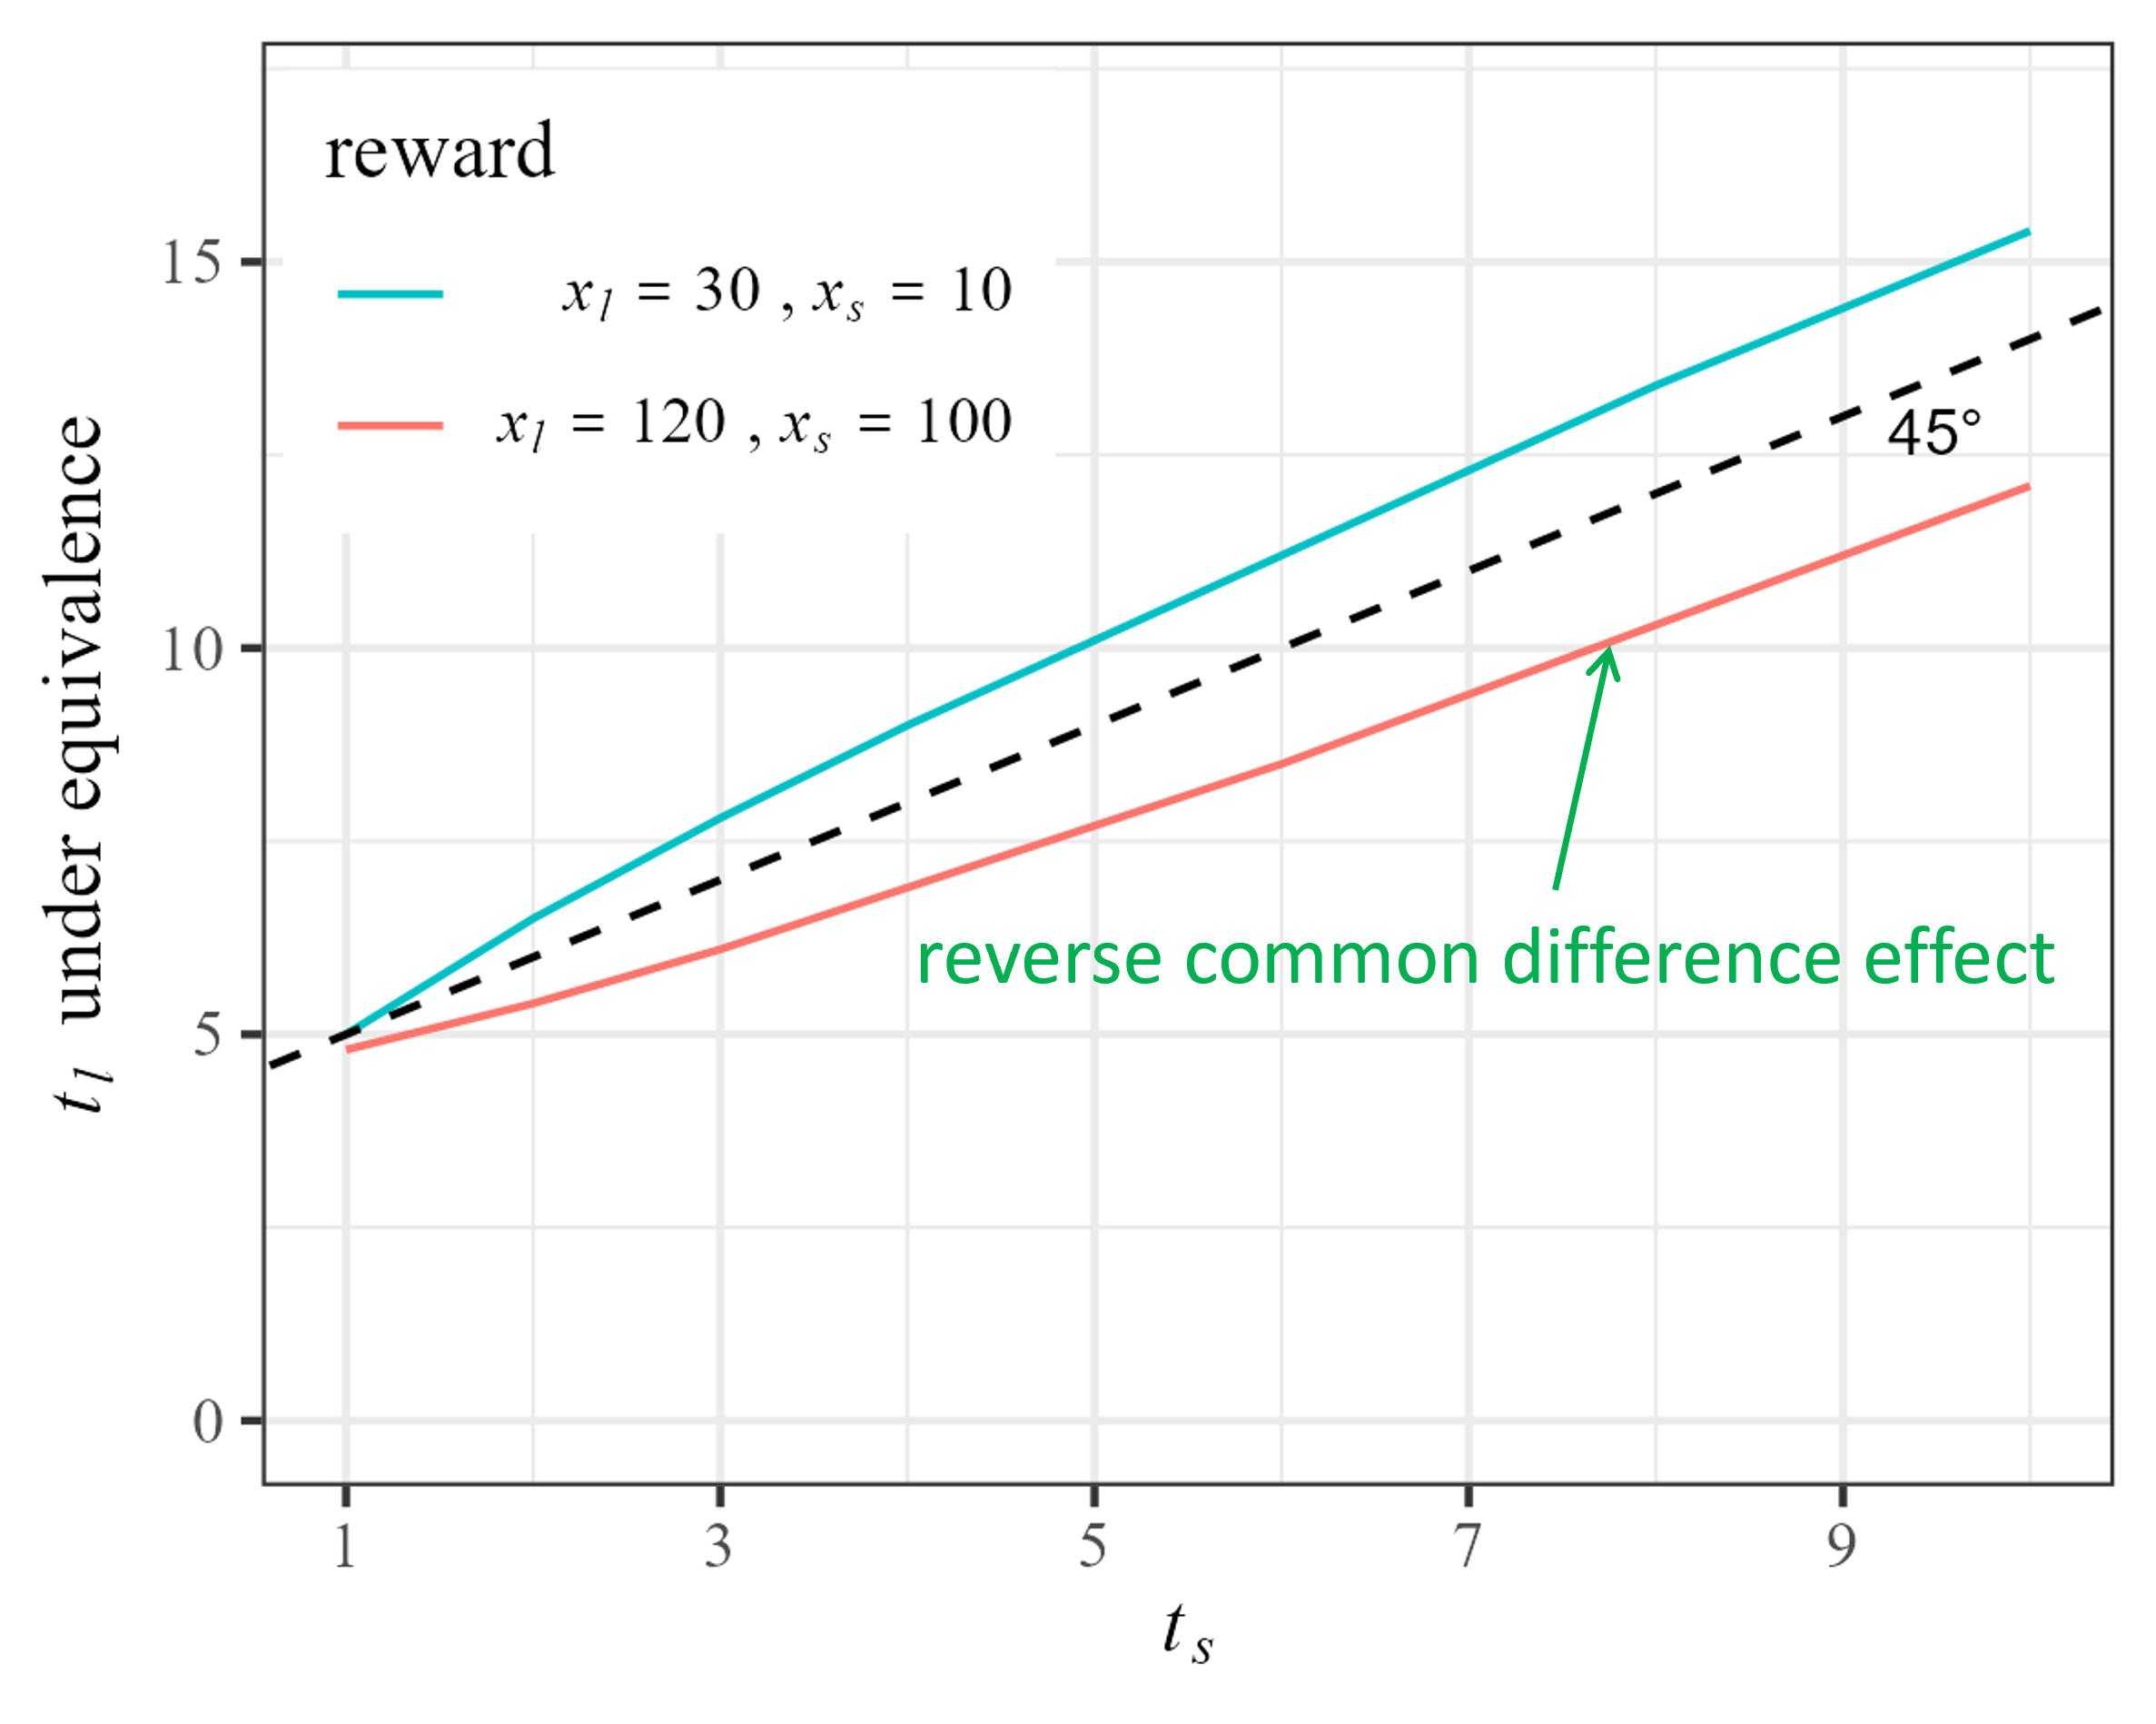
\includegraphics[width=0.65\textwidth]{figures/common_diff.png}   
  \caption{The common difference effect and its reverse}
  \vspace{8pt}
  \begin{minipage}{1.0\textwidth}
{\par\footnotesize Note: $x_l$ and $x_s$ are the positive reward levels for LL and SS. The values of LL and SS are calculated based on Equation (4). $d_t=0.75^t$, $u(x)=x^{0.6}$, $\lambda=2$. For each level of $t_s$, we identify the delay $t_l$ that makes the value of LL equivalent to SS. The blue line (above) demonstrates the common difference effect, and the red line (below) demonstrates the reverse common difference effect.}
\end{minipage}
  \label{fig:common_diff} 
\end{figure}

Figure \ref{fig:common_diff} demonstrates an example for the reverse
common difference effect. In the figure, we set \(v_s=x_s^{0.6}\),
\(v_l=x_l^{0.6}\), \(\delta=0.75\), \(\lambda=2\). For each level of the
delay \(t_s\), we identify the longer delay \(t_l\) that makes the value
of LL equivalent to SS. If the common different effect is valid,
increasing \(t_s\) and \(t_l\) by the same level would make the DM
prefer LL. Under this condition, for one unit increase in \(t_s\), to
make LL and SS valued equally, the identified \(t_l\) should be
increased by a time greater than one unit. On the contrary, if the
reverse common difference effect is valid, for one unit increase in
\(t_s\), the identified \(t_l\) should be increased by a time smaller.
In Figure \ref{fig:common_diff}, the blue line (above) reflects the
common different effect, while the red line (below), which has a lower
\(v_l-v_s\) and \(v_l/v_s\), reflects the reverse of it.

\hypertarget{concavity-of-discount-function}{%
\subsection{Concavity of Discount
Function}\label{concavity-of-discount-function}}

Many time discounting models, such as exponential and hyperbolic
discounting, assume the discount function is convex in time delay. This
type of discount function predicts DM is \emph{risk seeking over time
lotteries}. To illustrate, suppose a reward of level \(x\) is delivered
at period \(t_l\) with probability \(\pi\) and is delivered at period
\(t_s\) with probability \(1-\pi\), where \(0<\pi<1\). Meanwhile,
another reward of the same level is delivered at period \(t_m\), where
\(t_m=\pi t_l +(1-\pi) t_s\). Under such discount functions, the DM
should prefer the former reward to the latter reward. For instance, she
may prefer receiving an amount of money today or in 20 weeks with equal
chance, rather than receiving it in 10 weeks with certainty. However,
experimental studies suggest that people are often \emph{risk averse
over time lotteries}, i.e.~they prefer the reward to be delivered at a
certain time \citep{onay2007intertemporal, dejarnette2020time}.

One way to accommodate risk aversion over time lotteries is to make the
discount function concave in terms of delay. Notably,
\citet{onay2007intertemporal} find that people are more likely to be
risk averse over time lotteries when \(\pi\) is small, and to be risk
seeking when \(\pi\) is large. Given that \(t_m\) is increasing in
\(\pi\), we can claim that the discount function should be concave in
delay for the near future but convex for the far future.
\citet{takeuchi2011non} find the supportive evidence for this shape of
discount function. In Proposition 3, we apply Equation (4) and show that
the AMD model produces this shape of discount function when the DM is
impatient and the reward level \(x\) is large enough.

\noindent \textbf{Proposition 3}: \emph{Suppose a single reward} \(x\)
is \emph{delivered at period} \(T\)\emph{. Let} \(w_T\) \emph{denote the
AMD factor for this reward. If} \(\delta =1\)\emph{, then} \(w_T\)
\emph{is convex in} \(T\)\emph{. If} \(0<\delta<1\)\emph{, there exist a
reward threshold} \(\underline{x}>0\) \emph{and a time threshold}
\(\underline{T}>0\) \emph{such that:}

\begin{enumerate}
\def\labelenumi{(\alph{enumi})}
\tightlist
\item
  \emph{when} \(x\leq \underline{x}\)\emph{,} \(w_T\) i\emph{s convex
  in} \(T\);
\item
  \emph{when} \(x > \underline{x}\)\emph{,} \(w_T\) i\emph{s convex in}
  \(T\) \emph{given} \(T\geq \underline{T}\)\emph{, and it is concave
  in} \(T\) \emph{given} \(0<T<\underline{T}\)\emph{.}
\end{enumerate}

The proof of Proposition 3 is in Appendix C. Figure
\ref{fig:discount_value_function}(a) demonstrates the convex discount
function (blue line, below) and the inverse-S shaped discount function
(red line, above) that could be yielded by Equation (4).

\begin{figure}[h]
    \centering
    \begin{subfigure}{0.49\textwidth}
        \centering
        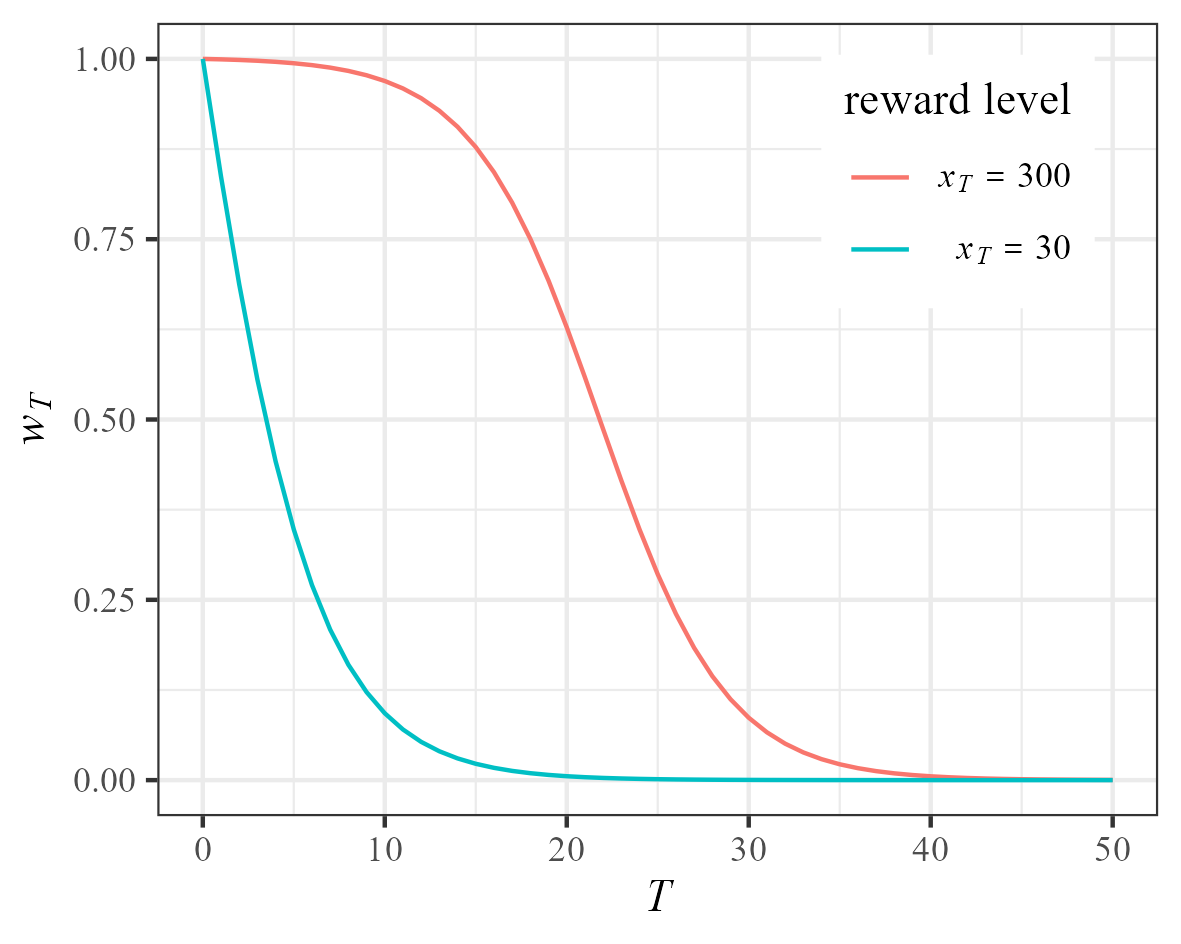
\includegraphics[width=\linewidth]{figures/concave_discount.png} 
        \caption{discount function}
    \end{subfigure}
    \hfill
    \begin{subfigure}{0.49\textwidth}
        \centering
        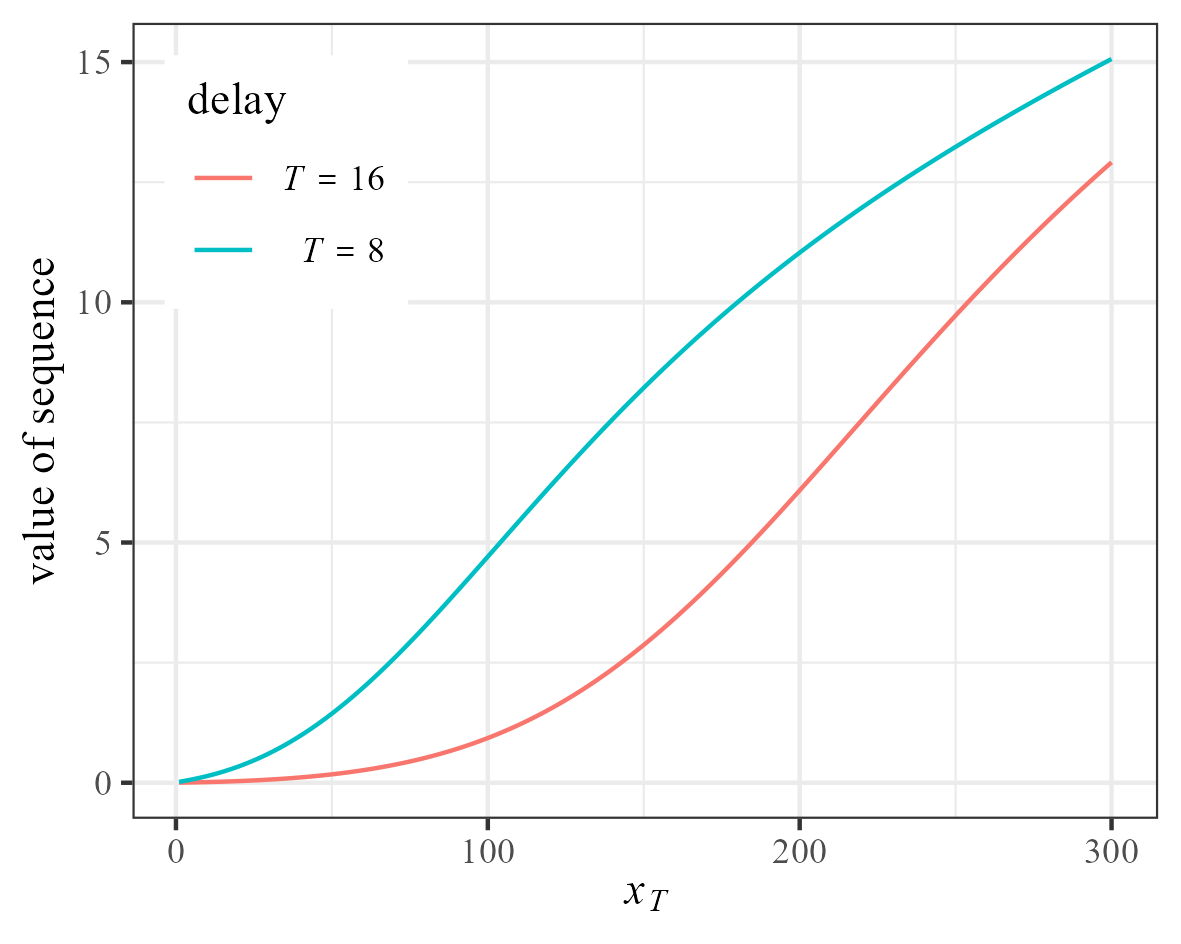
\includegraphics[width=\linewidth]{figures/s_shape_value.png}
        \caption{value function}
    \end{subfigure}
    \caption{Discount function and value function for a delayed reward}

  \vspace{8pt}
  \begin{minipage}{1.0\textwidth}
{\par\footnotesize Note: A reward of level $x_T$ is delivered at period $T$. The discount function and value function are calculated based on Equation (4). $d_t=0.75^t$, $u(x)=x^{0.6}$, $\lambda=2$.}
\end{minipage}
    
    \label{fig:discount_value_function}
\end{figure}

\hypertarget{s-shaped-value-function}{%
\subsection{\texorpdfstring{S-Shaped Value Function
\label{s_shape_value}}{S-Shaped Value Function }}\label{s-shaped-value-function}}

A common assumption in decision theories for the instantaneous utility
function \(u(.)\) is \(u''<0\). Usually, this implies the value function
of a reward is concave. However, empirical evidence suggests that the
value functions are often S-shaped. Such S-shaped value functions can be
generated by various sources, such as reference dependence
\citep{kahneman1979prospect} and efficient coding of numbers
\citep{louie2012efficient}. Through the AMD model, we provide a novel
account for S-shaped value function based on the insight that larger
rewards capture more attention.

Consider a reward of level \(x\) delivered at period \(T\). Its value
function can be represented by \(U(x,T)=w_T(x)u(x)\). We assume
\(u'>0\), \(u''<0\), and \(w_T\) is determined by Equation (4). \(w_T\)
is increasing with \(x\) as the DM tends to pay more attention to larger
rewards. Both functions \(u(x)\) and \(w_T(x)\) are concave in \(x\); so
when \(x\) is small, they both grow fast. At some conditions, it is
possible that the product of the two functions is convex in \(x\) when
\(x\) is small enough. We derive the conditions for the S-shaped value
function in Proposition 4.

\noindent \textbf{Proposition 4}: \emph{Suppose} \(T\geq1\)\emph{,}
\(\frac{d}{dx}\left(\frac{1}{v'(x)}\right)\) \emph{is continuous in}
\((0,+\infty)\)\emph{, then:}

\begin{enumerate}
\def\labelenumi{(\alph{enumi})}
\item
  \emph{There exists a threshold} \(\bar{x} \in\mathbb{R}_{\geq0}\)
  \emph{such that} \(U(x,T)\) \emph{is strictly concave in} \(x\)
  \emph{when} \(x\in [\bar{x},+\infty)\).
\item
  \emph{If} \(\frac{d}{dx}\left(\frac{1}{v'(x)}\right)\) \emph{is
  right-continuous at} \(x=0\) \emph{and}
  \(\frac{d}{dx}\left(\frac{1}{v'(0)}\right)<1\)\emph{, there exists}
  \(x^*\in(0, \bar{x})\) \emph{such that, for any}
  \(x\in (0,x^*)\)\emph{,} \(U(x,T)\) \emph{is strictly convex in}
  \(x\).
\item
  \emph{There exists a threshold} \(\lambda^*\) \emph{and an interval}
  \((x_1,x_2)\) \emph{such that, if} \(\lambda<\lambda^*\)\emph{, for
  any} \(x\in(x_1,x_2)\)\emph{,} \(U(x,T)\) \emph{is strictly convex in}
  \(x\)\emph{, where} \(\lambda^*>0\) \emph{and}
  \((x_1,x_2)\subset(0,\bar{x})\)\emph{.}
\end{enumerate}

The proof of Proposition 4 is in Appendix D. Proposition 4 implies, if
the derivative of \(\frac{1}{v'(x)}\) converges to a small number when
\(x\rightarrow 0^+\), or the unit cost of attention reallocation
\(\lambda\) is small enough, the value function \(U(x,T)\) will be an
S-shaped in some interval of \(x\). Figure
\ref{fig:discount_value_function}(b) demonstrates two examples of this
S-shaped value function.

\hypertarget{intertemporal-correlation-aversion}{%
\subsection{Intertemporal Correlation
Aversion}\label{intertemporal-correlation-aversion}}

Consider a DM facing two lotteries, \(L1\) and \(L2\). For lottery
\(L1\), she can receive £100 today and £100 in 30 weeks with probability
1/2, and receive £3 today and £3 in 20 weeks with probability 1/2. For
lottery \(L2\), she can receive £3 today and £100 in 30 weeks with
probability 1/2, and receive £100 today and £3 in 20 weeks with
probability 1/2. In lottery \(L1\), rewards delivered at the two
different periods are positively correlated; in lottery \(L2\), those
rewards are negatively correlated. The expected discounted utility
theory predicts the DM is indifferent between the two lotteries.
However, recent studies find the evidence of \emph{intertemporal
correlation aversion}
\citep{andersen2018multiattribute, rohde2023intertemporal}. That is,
people often prefer lottery \(L2\) to \(L1\).\footnote{For theoretical
  analysis about intertemporal correlation aversion, please see
  \citet{epstein1983stationary}, \citet{epstein1989substitution},
  \citet{weil1990nonexpected}, \citet{bommier2005risk}, and
  \citet{bommier2017monotone}. The AMD model takes a similar form to the
  class of models defined by \citet{epstein1983stationary}. A key
  feature of such models is that the discount factor for future
  utilities is dependent on the utility achieved in the current period.}

For the above example, intertemporal correlation aversion can be
explained by the AMD model as follows. The model assumes the allocation
of decision weights is within each certain reward sequence, which
implies the DM would first aggregate values over time in each state and
then solve the certainty equivalence. For simplicity, suppose there are
only two periods. In the state that the DM receives £3 in two periods,
suppose she allocates decision weight \(w\) to the first period and
\(1-w\) to the second period. Note when \(u(s_0)=u(s_1)=...=u(s_T)\),
the AMD factor for every period \(t\) remains the same as its default
discount factor \(d_t\). So, in the state that the DM receives £100 in
two periods, the decision weights is also the same as \(w\) and \(1-w\).
In the state that the DM can receive £100 in the first period and £3 in
the second period, the reward of £100 can capture more attention so that
its decision weight, say \(w'\), is greater than \(w\). Similarly, in
the state that the DM receives £3 earlier and then £100, the decision
weight for the later reward £100, say \(1-w''\), is greater than
\(1-w\). Therefore, the value of the lottery in which rewards are
positively correlated, can be represented by
\(0.5\cdot u(3)+0.5\cdot u(100)\). Whereas, for the lottery in which
rewards are negatively correlated, the value can be represented by
\(0.5(1-w'+w'')\cdot u(3)+0.5(1-w''+w')\cdot u(100)\). Given
\((1-w'')+w'>1-w+w=1\), the decision weight assigned to \(u(100)\),
which is \(0.5(1-w''+w')\), should be greater than 0.5. As a result, the
DM prefer the latter lottery than the former lottery.

In a more general setting, whether the AMD model can robustly produce
intertemporal correlation aversion is influenced by \(\lambda\). To see
this, we adopt the same definition of intertemporal correlation aversion
as \citet{bommier2005risk}. Let \((s_1,s_2)\) denote the result of a
lottery in which the DM can receive reward \(s_1\) in period \(t_1\) and
then reward \(s_2\) in period \(t_2\), where \(t_2>t_1\geq 0\). The
results of each lottery is of the same length of sequence. \(L1\)
generates \((x_s,y_s)\) and \((x_l,y_l)\) with equal chance, \(L_2\)
generates \((x_s,y_l)\) and \((x_l,y_s)\) with equal chance,
\(x_l>x_s>0\), \(y_l>y_s>0\). By Proposition 5, we show that in this
setting, we can always find a \(\lambda\) that makes the DM
intertemporal correlation averse.

\noindent \textbf{Proposition 5}: \emph{Suppose} \(U(L1), U(L2)\)
\emph{are the values of lotteries} \(L1\) \emph{and} \(L2\)
\emph{calculated based on the AAD model. For any} \(x_l>x_s>0\)\emph{,}
\(y_l>y_s>0\)\emph{, any default discount factors, and any time length
of lottery results, there exists} \emph{a threshold} \(\lambda^{**}\)
such that for all unit co\emph{st of attention reallocation}
\(\lambda\in(\lambda^{**},+\infty)\)\emph{, we have}
\(U(L1)<U(L2)\)\emph{, i.e.~the DM performs intertemporal correlation
aversion.}

The proof of Proposition 5 is in Appendix E. The threshold
\(\lambda^{**}\) is jointly determined by \(x_l\), \(y_l\), \(y_s\), as
well as the default discount factors for rewards delivered at \(t_1\)
and \(t_2\). Notably, when \(\lambda \leq \lambda^{**}\), the DM may be
intertemporal correlation seeking under some conditions.\footnote{To
  validate, one can set \(u(x_s)=5\), \(u(x_l)=10\), \(u(y_s)=1\),
  \(u(y_l)=3\). Suppose the results of each lottery contain only two
  periods, \(t_1\) and \(t_2\), and the default discount factors are
  uniformly distributed, i.e.~\(d_{t_1}=d_{t_2}\). In this case, setting
  \(\lambda=1\) would generate intertemporal correlation seeking, while
  setting \(\lambda=100\) would generate intertemporal correlation
  aversion.} This suggests a potentially new mechanism for intertemporal
correlation aversion, that is, DM performs intertemporal correlation
aversion because she attends more to larger rewards while attention
reallocation is very costly.

\hypertarget{concentration-bias}{%
\subsection{Concentration Bias}\label{concentration-bias}}

In the existing literature, one approach to applying attention in
intertemporal choice research is the focus-weighted utility model,
proposed by \citet{kHoszegi2013model}. In their model,
\citeauthor{kHoszegi2013model} assume that within a reward sequence, the
decision weight for a reward is increasing with the difference of that
reward from a reference point.\footnote{In this paper, we take zero
  reward as the reference point for every period. So, this assumption is
  also true for the AMD model.} The model predicts that people may
perform a \emph{concentration bias} and
\citet{dertwinkel2022concentration} find supportive evidence for such a
prediction. In this subsection, we show that the AMD model provides an
alternative way to generate the concentration bias. Furthermore, we
identify the conditions in terms of impatience and attention
reallocation cost, which are beyond the predictions of
\citet{kHoszegi2013model}, for the concentration bias.

To illustrate the concentration bias, consider a DM with a consumption
budget £100 to spend over four days (from period 0 to period 3). Suppose
the DM has two options: concentrating all consumption at period 0, or
splitting the consumption evenly over four periods. The concentration
bias implies that she would prefer the first option to the second. We
denote the first option as sequence {[}100,0,0,0{]} and the second
option as sequence {[}25,25,25,25{]}. For convenience, we assume the
default discount factor for any period \(t\) is \(d_t = \delta^t\) and
\(0<\delta<1\). According to the AMD model, the DM prefers the first
option if and only if\[
\frac{e^{u(100)/\lambda}}{e^{u(100)/\lambda}+\delta+\delta^2+\delta^3}\cdot u(100)>u(25)
\]Obviously, this inequality holds only when \(\delta\) or \(\lambda\)
is small enough, which implies the DM should be very impatient or she
can reallocate attention at a very low cost. Notably, under the AMD
model, it is also possible that the DM prefers concentrating all
consumption at the final period, i.e.~the sequence {[}0,0,0,100{]}, to
the second option {[}25,25,25,25{]}. In this case, the decision weight
multiplied by \(u(100)\) in the inequality would become
\(\frac{\delta^3 \exp\{u(100)/\lambda\}}{1+\delta+\delta^2+\delta^3 \exp\{u(100)/\lambda\}}\).
Then, the inequality holds only when both \(\delta\) is large enough and
\(\lambda\) is small enough. Both cases are in line with the claim in
\citet{kHoszegi2013model} and \citet{dertwinkel2022concentration} that
the concentration bias can make people behave too impatiently or too
patiently.

Next, we derive the conditions for concentration bias in a general
optimal-decision setting. From the above example we can draw an
intuition that, in a general case, to observe the concentration bias we
require the unit cost of attention reallocation \(\lambda\) to be small.
We show in Proposition 6 that this intuition is true. Suppose the DM has
a consumption budget \(m\) (\(m>0\)) to spend over \(T\) periods. Let
reward sequence \(s_{0\rightarrow T}\) represent her consumption plan at
period 0, and let \(A\subset \mathbb{R}_{\geq 0}^{T+1}\) denote her
alternative space. In period 0, DM wants to find a
\(s_{0\rightarrow T}\) to solve the optimization problem:\[\tag{5}
\max_{s_{0\rightarrow T}\in A}\;\sum_{t=0}^T w_t u(s_t)\\ 
\]where\[
A=\left\{s_{0\rightarrow T} \bigg|\;\sum_{t=0}^T s_t = m,\; \forall t:s_t \geq 0\right\}
\]and \(w_t\) is the AMD factor for consumption in period \(t\), subject
to default discount factor \(d_t\). For \(s\in[0,m]\), we have
\(0<u'(s)<\infty\), \(-\infty<u''(s)<0\). Henceforth, we denote the
optimization problem in Equation (5) by
\(\mathcal{O}(m,A,\{d_t\}_{t=0}^T)\). By Proposition 6, we know as long
as the DM is impatient (for all period \(t<T\), we have
\(d_t>d_{t+1}>0\)) and \(\lambda\) is small enough, her optimal
consumption plan is to consume all of \(m\) immediately. The proof of
Proposition 6 is in Appendix F.

In Section \ref{model_setting}, we state that the unit cost of attention
reallocation \(\lambda\) has a potential link to cognitive uncertainty.
If the DM is highly certain that the default discount factors
\(\{d_t\}_{t=0}^T\) truly capture her preference in the local context,
she may inhibit the learning about value signals and thus \(\lambda\)
should be high. This link is also helpful for understanding the
relationship between \(\lambda\) and concentration bias: when allocating
a budget over time, if the DM is totally uncertain about what to do (so
\(\lambda\) is very small), she may simply concentrate her budget into
one period and consume it all.

\noindent \textbf{Proposition 6}: \emph{Suppose the DM faces the
planning problem} \(\mathcal{O}(m,A,\{d_t\}_{t=0}^T)\), \emph{and for
all period} \(t<T\), we have \(d_t >d_{t+1}>0\)\emph{.} \emph{There
exists a threshold} \(\underline{\lambda}>0\) \emph{such that for any}
\(\lambda\leq\underline{\lambda}\)\emph{, her optimal consumption plan
is to concentrate all consumption at period 0.}

\hypertarget{inconsistent-planning-and-learning}{%
\subsection{\texorpdfstring{Inconsistent Planning and Learning
\label{inconsistent}}{Inconsistent Planning and Learning }}\label{inconsistent-planning-and-learning}}

An extensive amount of research evidence suggests that people often
exhibit time-inconsistent behaviors in their daily lives
\citep{ericson2019intertemporal}. For example, they often consume more
than they originally planned, and procrastinate on effortful tasks. In a
general sense, such behaviors can be termed present-biased behaviors.
Several theories have been proposed for explaining the present-biased
behaviors, such as dual-system preferences \citep{laibson1997golden},
naivete \citep{o1999doing}, reference dependence
\citep{kHoszegi2009reference}, and optimistic beliefs
\citep{brunnermeier2017optimal}. Based on the AMD model, we can provide
an alternative explanation for these behaviors: in dynamic
decision-making, people update their default discount factors over time.
In more intuitive terms, during each decision step, people will
reference their past experiences when allocating attention. If, in the
last step, they allocate too much attention to a particular period, they
may then take this as a given or default status in the following step
and continue to add attention to it. Compared with the existing
theoretical explanations, our explanation is built on learning and
memory. To perform present-biased behaviors, the DM should recall her
mental status at the end of the last step and learn how to allocate
attention accordingly. A memoryless DM may perform the reverse behavior.
We analyse this with the consumption planning problem in the last
subsection.

Again, we suppose the DM has a budget \(m\) for consumption. She needs
to allocate it over \(T\) periods (\(T\geq 2\)) and the end of sequence
is a fixed date. In period 0, her default discount factors
\(\{d_t\}_{t=0}^T\) satisfy \(d_t>d_{t+1}>0\), where \(t<T\). When
making consumption plan, she would initially weight consumption of
period 1 higher than consumption of any other future period. So, she may
naturally plan to consume more in period 1 than in period \(t=2,…,T\).
This in turn, makes her relatively attend more to period 1. Her optimal
consumption plan of period 0 should result in \(w_1/w_t>d_1/d_t\) for
each \(t=2,…,T\). When arriving in period 1, we assume the DM will use
the AMD factors determined in the last step as the new default discount
factors. This will lead her to initially weight consumption of period 1
even higher, and therefore create a motive for over-consumption. In the
end, her actual consumption in period 1 will be higher than what has
been planned in the last step. Such a trend could continue until she
reaches the final period or runs out of money.

\begin{figure}[h]
    \centering
    \begin{subfigure}{0.49\textwidth}
        \centering
        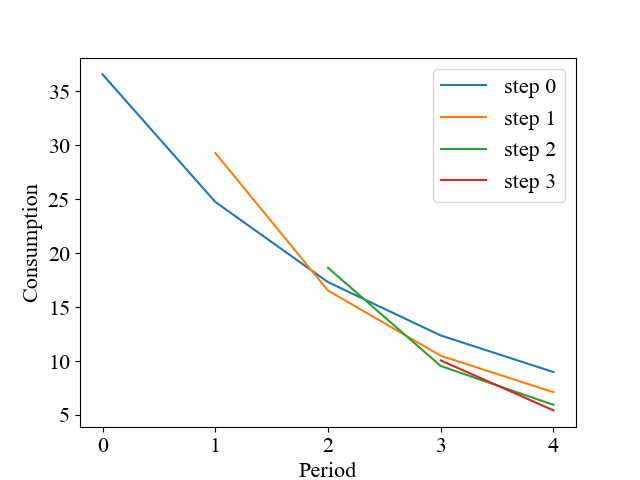
\includegraphics[width=\linewidth]{figures/learning_c.png} 
        \caption{with learning}
    \end{subfigure}
    \hfill
    \begin{subfigure}{0.49\textwidth}
        \centering
        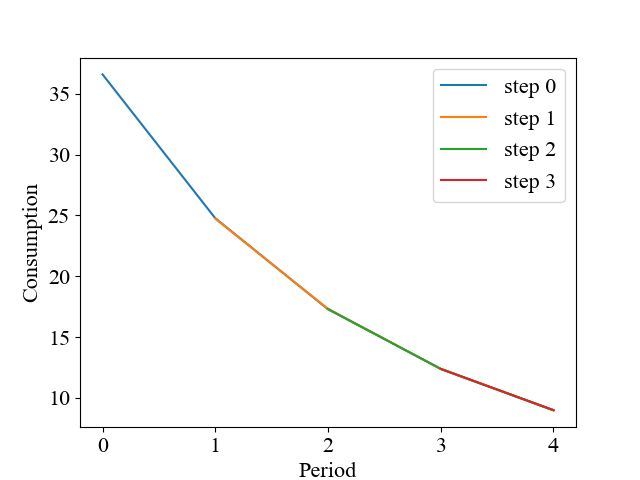
\includegraphics[width=\linewidth]{figures/no_learning_c.png}
        \caption{without learning}
    \end{subfigure}
    \caption{Optimal Consumption Plan Over Time}

  \vspace{8pt}
  \begin{minipage}{1.0\textwidth}
{\par\footnotesize Note: In step 0, the DM allocates consumption budget $m=100$ over periods 0-4. In step 1, she allocates the remaining consumption over periods 1-4, and so on. "with learning" means the DM updates default discount factors per step; "without learning" means the default discount factors are constant over time. $d_t^0=0.9^t$, $u(x)=x^{0.6}$, $\lambda=70$. Each optimization problem is solved by projection gradient descent method.}
\end{minipage}
    
    \label{fig:inconsistency_learning}
\end{figure}

Figure \ref{fig:inconsistency_learning} illustrates the relationship
between time inconsistency and learning. In the figure, we set
\(u(x)=x^{0.6}\), \(T=4\), \(\lambda=70\). At the first step of
planning, the DM has a budget of \(m=100\) for consumption and her
default discount factors are exponential: \(d_t^0=0.9^{t}\). Under the
condition ``with learning'', which means the DM takes AMD factors of the
optimal consumption plan as default discount factors for the next step,
we observe a tendency for over-consumption. Under the condition
``without learning'', which means the default discount factors are
constant over time, the DM's behavior is closer to being
time-consistent, and in each step, the actual consumption is slightly
lower than the consumption planned one step earlier.\footnote{In one
  simulation under the condition ``without learning'', in step 0, the DM
  plans to consume 24.76 in period 1, and she ends up consuming 24.74.
  Also, in step 1, she plans to consume 17.32 in period 2, and she ends
  up consuming 17.31.}

We state these results formally in Proposition 7. We focus on the
transition from period 0 to period 1, but the conclusions can be
expanded to other periods. When the DM plans her consumption in period
\(j\) (\(j=0,1\)), the default discount factor for period \(t\) is
termed \(d_t^j\) and the corresponding AMD factor is termed \(w^j_t\),
where \(t\geq j\). In the period 0's optimal consumption plan, the DM
plans to consume \(s_t^*\) in period \(t\), and in the period 1's
optimal plan, she plans to consume \(s_t^{**}\). The alternative space
is \(A\) in period 0 and becomes \(A'\) in period 1. Notably, to make
the time-inconsistency results hold, the DM should not concentrate all
consumption into period 0. From Proposition 6, we know that it requires
\(\lambda\) to be large enough. The proof of Proposition 7 is in
Appendix G.

\noindent \textbf{Proposition 7}: \emph{Suppose the DM faces the
planning problem} \(\mathcal{O}(m,A,\{d^0_t\}_{t=0}^T)\) \emph{in period
0 and} \(\mathcal{O}(m-s_0^*,A',\{d_t^1\}_{t=1}^T)\) \emph{in period 1.}
\emph{There exists a threshold} \(\bar{\lambda}>\underline{\lambda}\)
\emph{such that when} \(\lambda\in[\bar{\lambda},+\infty)\)\emph{, the
following is true:}

\begin{enumerate}
\def\labelenumi{(\alph{enumi})}
\item
  \emph{In period 0, for any sequence}
  \(s_{0\rightarrow T}^*\in \{s_{0\rightarrow T}|s_{0\rightarrow T}\in A,\forall t<T:s_t>s_{t+1}>0\}\)\emph{,
  there exist a specification of default discount factors}
  \(\{d_t^0\}_{t=0}^T\), where \emph{for all} \(t<T\) \emph{we have}
  \(d_t^0 >d_{t+1}^0>0\), \emph{such that} \(s_{0\rightarrow T}^*\)
  \emph{is the optimal consumption plan.}
\item
  \emph{Given} \(s_{0\rightarrow T}^*\) \emph{as the period 0's optimal
  consumption plan, if in period 1, for all} \(t\geq 1\) \emph{we have}
  \(d_t^1=d_t^0\)\emph{, then there must be} \(s_1^{**}< s_1^*\)\emph{;
  if instead we have} \(d_t^1=w_t^0\)\emph{, then}
  \(s_1^{**}> s_1^*\)\emph{.}
\end{enumerate}

In the part (a) of Proposition 7, we select an interior solution for the
consumption planning problem in period 0. The part (b) suggests that if
we do not take into account the updating of default discount factors,
the DM would perform under-consumption behavior over time. In reverse,
assuming the default discount factors are updated based on the AMD
factors of the most recent consumption plan will result in
over-consumption behavior. The former reflects the behavior of a DM
``without learning'', while the latter reflects how the DM would behave
``with learning''.

\hypertarget{discussion}{%
\section{\texorpdfstring{Discussion
\label{discuss}}{Discussion }}\label{discussion}}

\hypertarget{selection-of-sequence-length}{%
\subsection{\texorpdfstring{Selection of Sequence Length
\label{seq_length}}{Selection of Sequence Length }}\label{selection-of-sequence-length}}

In our model, the attention a DM can allocate to each time period is
affected by sequence length. When a sequence contains more periods, the
average attention she can allocate to each period naturally decreases.
In Section \ref{hidden_zero}, we discuss how this can generate the
hidden zero effect. Nevertheless, in reality, we usually cannot observe
the actual sequence length perceived by the people. Researchers using
our model need to make their own assumptions about sequence length. In
this subsection, we discuss two issues related to setting these
assumptions and provide recommendations.

The first issue is about the unit of time. A given duration can be
represented as sequences of different lengths depending on the time unit
used, such as months or days. For example, ``receive £10 in 1 month''
and ``receive £10 in 30 days'' essentially mean the same thing, but the
latter seems to involve more units of time. When represented in
sequence, the former can be represented by {[}0,10{]}, and the latter
can be {[}0,0,\ldots,0,10{]}, with 30 zeros before the 10. In
``standard'' discounting models, the number of zeros before the 10 has
no effect on the valuation of the sequence. Whereas, the AMD model
predicts that, when the reward sequence is described with more time
units, the DM may perceive the waiting period for the £10 payment as
longer, thereby discounting its value to a greater extent.

As an illustration, in the exponential discounting model, suppose each
period represents a month and the discount factor for period \(t\) is
\(\delta^t\). The value of sequence {[}0,10{]} could be written as
\(\delta \times u(10)\). For the sequence {[}0,0,\ldots,0,10{]}, which
includes 30 zeros where each period represents a day, we can convert the
monthly discount rate to a daily discount rate. Thus, the discount
factor for period \(t\) becomes \(\delta^{\frac{1}{30}\cdot t}\), and
the value of sequence is still the same. However, this approach does not
apply to the AMD model. In the AMD model, suppose the default discount
factors are exponential, as we have stated. According to Equation (4),
the discount factor for the £10 payment is \(1/(1+G(T)e^{-v(10)})\). And
in the former case \(G(T)=\delta^{-1}\), while in the latter case
\(G(T)=\delta^{-1}+\delta^{-\frac{29}{30}}+...+\delta^{-\frac{1}{30}}\).
If we use the same parameterization in both cases, then in the latter
case, the value of the £10 payment should be more discounted.\footnote{If,
  in reverse, we elicit the DM's time preference from experiments and
  model it using the sequence with 30 zeros, then the estimate for
  \(\delta\) should be greater compared to the sequence with only one
  zero.}

The AMD model's prediction that people perceive the sequence with more
time units as longer is also consistent with the numerosity effect. This
effect refers to the tendency to overestimate quantity based on the
number of units presented \citep{pelham1994easy} and has been
extensively studied in various fields, particularly in consumer behavior
\citep{zhang2012and, monga2012years}.\footnote{Some of such studies,
  such as \citet{monga2012years}, state that the unit itself can also
  influence decisions. For example, people may perceive ``month'' as
  longer than ``day''. So, the sequence that takes each month as a
  period may correspond to a smaller \(\delta\).} To the best of our
knowledge, there is currently no clear evidence of the numerosity effect
in intertemporal choice. Nonetheless, this can be a potential direction
for future research. To capture such an effect, we recommend that
researchers choose sequence lengths that match the time units presented
to participants. For the given example, if a reward sequence is
expressed as ``receive £10 in 1 month'', researchers would better
represent it as {[}0,10{]} rather than a sequence with 30 zeros.

The second issue is about the end of sequence. In our explanation of the
model's implications, an implicit assumption is that each sequence
terminates at the period when the final positive reward is delivered.
For example, for a sequence described by ``receive £10 in 1 month'', we
represent it as {[}0,10{]} rather than {[}0,10,0,0{]}. This assumption
is sufficient for most of the well-established psychological effects in
intertemporal choice. However, under this assumption the model is
incapable of distinguishing between two constant sequences of different
lengths. As an illustration, consider a choice between two options: (A)
``receive £10 now''; and (B) ``receive £10 now, plus £10 in 1 month,
plus £10 in 2 months''. According our implicit assumption, option (A)
can be represented by a single-period sequence {[}10{]} and option (B)
can be represented by {[}10,10,10{]}. In reality, people will definitely
prefer option (B) to (A). But, as the AMD model assumes a constant sum
of decision weights, such representations would result in both options
being equally valued at \(u(10)\).

We propose two remedies for this issue. The simplest approach is to
assume that the DM always takes into account one additional period when
processing each sequence. For example, she represents option (A) as
{[}10,0{]} and option (B) as {[}10,10,10,0{]}. Then, in option (B), the
attention jointly captured by the three 10s must be greater than the
attention captured by the single 10 in option (A).\footnote{Set
  \(u(x)=x^{0.6}\), \(d_t=0.9^t\), \(\lambda=2\). According to the AMD
  model, the value of option (A) is 3.55 and that of option (B) is 3.84.}
In Appendix H, we show that adding a period to the end of each sequence
does not affect the implications of the model that we have discussed for
choice between sequences. In addition, a more complex way to address the
issue is to assume the sequences ends at a random position. Given that
we do not know how people would actually perceive the sequence length,
for option (B), we could assume the end of sequence follows a
distribution, ranging from the third period to infinity. Researchers
could set the class of distribution and then estimate its parameters
from the data, which would allow them to accommodate a wider range of
phenomena. We consider this as a potential direction for future
research.

To understand why including a zero (or zeros) at the end of a sequence
is psychologically plausible, we can examine how people would perceive
information that is not explicitly mentioned in each option. Adding a
certain period to a sequence implies the DM must pay some attention to
the reward delivered in that period, in order to process its value. For
option (B), the DM knows there will be no reward delivered after period
3, although this is not explicitly described. On the one hand, this
prohibits the DM from allocating more attention to perceive the value of
rewards delivered in the far future (such rewards are not included in
the sequence). On the other hand, ``no reward will be delivered after
period 3'' could be seen as additional information beyond what is
provided in option (B). In other words, the DM needs to at least
allocate some attention to processing such an information, and adding
some periods of no reward is a simple way to capture this.

\hypertarget{relation-to-other-intertemporal-choice-models}{%
\subsection{\texorpdfstring{Relation to Other Intertemporal Choice
Models
\label{relation_to_other}}{Relation to Other Intertemporal Choice Models }}\label{relation-to-other-intertemporal-choice-models}}

In the existing literature, the theory most similar to AMD is the
salience theory, originally proposed by \citet{bordalo2012salience}. A
recent review \citep{bordalo2022salience} summarizes the latest
developments in the theory. According to that theory, the ``salience''
of an element in a sequence is increasing with its deviation from a
reference point. Within the scope of this paper, we could set the
reference point to zero. Thus, the salience theory also predicts that
people pay more attention to large rewards and less attention to small
rewards. Moreover, in Section \ref{inconsistent}, we consider the role
of memory and learning in generating time-inconsistent behavior under
the AMD model. This is also related to \citet{bordalo2020memory}, which
incorporates a memory-based reference point in the salience theory.

Nevertheless, unlike the AMD model, the salience theory does not impose
any restrictions on the sum of decision weights; it merely re-normalizes
the decision weights. Through applying that theory to intertemporal
choice, the value of a sequence could be represented by
\(U=\sum_{t=0}^T \pi_tw_tu(s_t)\), where \(\pi_t\) is some ``standard''
discount factor (e.g.~the exponential discount factor
\(\pi_t=\delta^t\)), and the re-normalization weight \(w_t\) satisfies
\(\sum_{t=0}^T w_t=1\). As a result, given a sequence {[}100, 4{]},
additional two additional 4s to the end to make it {[}100, 4, 4, 4{]},
would have different consequences under salience theory compared to the
AMD model. In the salience theory, this may make the element 100 more
``salient'', as the total of decision weights increases from
\(\pi_0 + \pi_1\) to \(\pi_0 + \pi_1 + \pi_2 + \pi_3\), and the 100 can
capture the majority of this total. Whereas, in the AMD model, this
operation always reduces the attention allocated to each element.

Some other models also claim to incorporate attentional mechanisms in
intertemporal choice. For example, the focus-weighted utility theory
\citep{kHoszegi2013model} also assumes that people discount the value of
a large reward less because they focus on it more (if taking zero as the
reference point). Despite that, the focus-weighted utility theory does
not perform any normalization of decision weights.
\citet{steiner2017rational} examine the role of rational inattention in
dynamic risky decision-making, and use it to account for inertia and
status quo bias. That theory is grounded in the instrumental utility of
information while our model is grounded in its hedonic and cognitive
utilities (see Section \ref{interpretation}). In psychology, some
researchers use the attentional drift-diffusion model
\citep[aDDM, see][]{krajbich2010visual} to analyse choices between SS
and LL \citep{amasino2019amount}. In the aDDM, the value of an option is
subject to an evidence accumulation process. If the DM pays more
attention to an option (or attribute), she can accumulate more evidence
about its value, leading her to value it more. So far, studies about
aDDM have yet to examine how attention shifts within a sequence, but
they may relate to the cost of attention reallocation, which controls
the rate of information acquisition in the AMD model.

Moreover, the trade-off models for intertemporal choice provides an
alternative approach to model choices between sequences
\citep[\citet{scholten2016cumulative},
\citet{scholten2024unified}]{read2012tradeoffs}. Such models assume that
the DM trades off the average utility of receiving rewards against the
average disutility of waiting. Yet, they can still be expressed in a
form similar to additive discounted utilities. For example, in
\citet{scholten2016cumulative}, the value of a sequence can be
represented by \(U=\sum_{t=0}^T w_tu(s_t)\), where
\(w_t=1-\kappa\frac{T(T+1)(T-t+1)}{\sum_{\tau=0}^T (T-\tau+1)u(s_\tau)}\)
and \(\kappa\) is a positive parameter. Under this specification of
\(w_t\), increasing \(s_t\) can increase the decision weights for all
rewards in the sequence, while in the AMD model, this increases the
decision weight for \(s_t\) but reduces the decision weights for all the
other rewards.

\hypertarget{possible-improvements}{%
\subsection{Possible Improvements}\label{possible-improvements}}

There are several ways to improve our model. First, the DM may not just
allocate attention within a sequence, but also across sequences. As a
result, within the same choice set, the sum of decision weights for one
sequence may be smaller than that for another. Researchers interested in
this direction might also refer to \citet{manzini2014stochastic} and
\citet{gossner2021attention}. Second, as suggested by the aDMM, when the
DM focuses more on a reward, she may not only assign it greater weight,
but also accelerate the rate at which she learns about its value. In our
model, the learning rate is controlled by a unified parameter
\(\lambda\). But in reality, this parameter might vary across different
rewards as they capture different levels of attention.
\citet{leong2017dynamic} provide an example of analyzing both
consequences of attention simultaneously. Third, in the existing
literature, the softmax function is usually used to model stochastic
choices. Our model examines how this function can be used to study
mental representations of reward sequences. Future research could
explore its use in risk perception, and integrate these fields to offer
a unified behavioral economic framework for analyzing dynamic risky
decision-making problems.

\renewcommand\refname{Reference}
  \bibliography{reference.bib}

\newpage

\hypertarget{appendix}{%
\section*{Appendix}\label{appendix}}
\addcontentsline{toc}{section}{Appendix}

\hypertarget{a.-proof-of-proposition-1}{%
\subsection*{A. Proof of Proposition
1}\label{a.-proof-of-proposition-1}}
\addcontentsline{toc}{subsection}{A. Proof of Proposition 1}

We present the proof of sufficiency here. That is, if \(\succsim\) has
an optimal discounting representation and satisfies Axiom 1-4, then it
has an AMD representation.

\noindent \textbf{Lemma 1}: \emph{If Axiom 1 and 3 hold, for any}
\(s_{0\rightarrow T}\)\emph{, there exist} \(w_0, w_1, …, w_T > 0\)
\emph{such that}
\(s_{0\rightarrow T} \sim w_0 \cdot s_0 + ...+w_T\cdot s_T\)\emph{,
where} \(\sum_{t=0}^T w_t=1\)\emph{.}

\noindent \emph{Proof}: If \(T=1\), Lemma 1 is a direct application of
Axiom 3. If \(T\geq 2\), for any \(2\leq t\leq T\), there should exist
\(\alpha_t\in(0,1)\) such that
\(s_{0\rightarrow t}\sim \alpha_t\cdot s_{0\rightarrow t-1}+(1-\alpha_t)\cdot s_{t}\).
By state-independence and reduction of compound alternatives, we can
recursively apply such equivalence relations as follows:\[
\begin{aligned}
s_{0\rightarrow T} &\sim \alpha_{T-1}\cdot s_{0\rightarrow T-1} + (1-\alpha_{T-1})\cdot s_T \\
&\sim  \alpha_{T-1}\alpha_{T-2}\cdot s_{0\rightarrow T-2} + \alpha_{T-1}(1-\alpha_{T-2})\cdot s_{T-1} + (1-\alpha_{T-1})\cdot s_T \\
& \sim ...\\
& \sim w_0 \cdot s_0 + w_1\cdot s_1 +... +w_T\cdot s_T
\end{aligned}
\]where \(w_0=\prod_{t=0}^{T-1}\alpha_t\), \(w_T = 1-\alpha_{T-1}\), and
for \(0<t<T\),
\(w_t=(1-\alpha_{t-1})\prod_{\tau=t}^{T-1}\alpha_{\tau}\). It is easy to
show the sum of \(w_0,…,w_T\) is equal to 1. \emph{QED}.

Therefore, if Axiom 1 and 3 hold, for any reward sequence
\(s_{0\rightarrow T}\), we can always find a convex combination of all
its elements, such that the DM is indifferent between the reward
sequence and this convex combination. If \(s_{0\rightarrow T}\) is a
constant sequence, i.e.~all its elements are constant, then we can
directly assume \(\mathcal{W}\) is AMD-style. So henceforth, we discuss
whether AMD can apply to non-constant sequences.

By Lemma 2, we show adding a new reward to the end of
\(s_{0\rightarrow T}\) has no impact on the relative decision weights of
rewards in the original reward sequence.

\noindent \textbf{Lemma 2}: \emph{For any}
\(s_{0\rightarrow T+1}\)\emph{, if}
\(s_{0\rightarrow T}\sim \sum_{t=0}^T w_t \cdot s_t\) \emph{and}
\(s_{0\rightarrow T+1} \sim \sum_{t=0}^{T+1} w'_t\cdot s_t\)\emph{,
where} \(w_t, w'_t>0\) and \(\sum_{t=0}^Tw_t=1\)\emph{,}
\(\sum_{t=0}^{T+1}w'_t=1\)\emph{, then when Axiom 1-4 hold, we can
obtain} \(\frac{w'_0}{w_0}=\frac{w'_1}{w_1}=…=\frac{w'_T}{w_T}\)\emph{.}

\noindent \emph{Proof}: According to Axiom 3, for any
\(s_{0\rightarrow T+1}\), there exist \(\alpha,\zeta \in (0,1)\) such
that\[\tag{A1}
\begin{aligned}
s_{0 \rightarrow T}\sim\alpha\cdot s_{0 \rightarrow T-1} + (1-\alpha)\cdot s_T \\
s_{0\rightarrow T+1} \sim \zeta\cdot s_{0\rightarrow T} + (1-\zeta)\cdot s_{T+1}
\end{aligned}
\]On the other hand, we drawn on Lemma 1 and set\[\tag{A2}
s_{0\rightarrow T+1} \sim \beta_0\cdot s_{0 \rightarrow T-1} + \beta_1\cdot s_T + (1-\beta_0-\beta_1)\cdot s_{T+1}
\]where \(\beta_0, \beta_1 > 0\). According to Axiom 4,
\(1-\zeta=1-\beta_0-\beta_1\). So, \(\beta_1=\zeta-\beta_0\). This also
implies \(\zeta > \beta_0\).

According to Axiom 2, we suppose there exists a reward sequence \(s\)
such that
\(s \sim \frac{\beta_0}{\zeta}\cdot s_{0 \rightarrow T-1} + (1-\frac{\beta_0}{\zeta})\cdot s_T\).
By Equation (A2) and reduction of compound alternatives, we have
\(s_{0\rightarrow T+1}\sim \zeta \cdot s + (1-\zeta)\cdot s_{T+1}\).
Combining Equation (A2) with the second line of Equation (A1) and
applying transitivity and state-independence, we obtain
\(s_{0\rightarrow T} \sim \frac{\beta_0}{\zeta}\cdot s_{0 \rightarrow T-1} + (1-\frac{\beta_0}{\zeta})\cdot s_1\).

We aim to prove that for any \(s_{0\rightarrow T+1}\), we can obtain
\(\alpha=\frac{\beta_0}{\zeta}\). We show this by contradiction.

Given the symmetry of \(\alpha\) and \(\frac{\beta_0}{\zeta}\), we can
assume that \(\alpha > \frac{\beta_0}{\zeta}\). Consider the case that
\(s_{0 \rightarrow T-1} \succ s_T\). By state-independence, for any
\(c\in \mathbb{R}_{\geq 0}\), we have
\((\alpha - \frac{\beta_0}{\zeta})\cdot s_{0\rightarrow T-1} + (1-\alpha+\frac{\beta_0}{\zeta})\cdot c \succ (\alpha - \frac{\beta_0}{\zeta})\cdot s_T + (1-\alpha+\frac{\beta_0}{\zeta})\cdot c\).
By Axiom 2, there exists \(z\in \mathbb{R}_{\geq 0}\) such that
\((1-\alpha)\cdot s_T + \frac{\beta_0}{\zeta}\cdot s_{0\rightarrow T-1}\sim z\).
Given \(c\) is arbitrary, we can set
\((1-\alpha+\frac{\beta_0}{\zeta})\cdot c \sim z\). By reduction of
compound alternatives, we can derive that\[
(\alpha-\frac{\beta_0}{\zeta})\cdot s_{0\rightarrow T-1} +(1-\alpha)\cdot s_T + \frac{\beta_0}{\zeta}\cdot s_{0\rightarrow T-1} \succ (\alpha-\frac{\beta_0}{\zeta})\cdot s_T +(1-\alpha)\cdot s_T + \frac{\beta_0}{\zeta}\cdot s_{0\rightarrow T-1}
\]where the LHS can be rearranged to
\(\alpha\cdot s_{0\rightarrow T-1} + (1-\alpha)\cdot s_T\), and the RHS
can be rearranged to
\(\frac{\beta_0}{\zeta}\cdot s_{0 \rightarrow T-1} + (1-\frac{\beta_0}{\zeta})\cdot s_1\).
They both should be indifferent from \(s_{0\rightarrow T}\). This
results in a contradiction.

Similarly, in the case that \(s_T \succ s_{0 \rightarrow T-1}\), we can
also derive such a contradiction. Meanwhile, when
\(s_{0\rightarrow T}\sim s_T\), \(\alpha\) and \(\frac{\beta_0}{\zeta}\)
can be any number within \((0,1)\). In that case, we can directly set
\(\alpha = \frac{\beta_0}{\zeta}\).

Thus, we have \(\alpha = \frac{\beta_0}{\zeta}\) for any
\(s_{0\rightarrow T+1}\), which indicates
\(\frac{\beta_0}{\alpha}=\frac{\beta_1}{1-\alpha}=\zeta\). We can
recursively apply this equality to any sub-sequence
\(s_{0\rightarrow t}\) (\(t\leq T\)) of \(s_{0\rightarrow T+1}\), so
that the lemma will be proved. \emph{QED}.

Now we move on to prove Proposition 1. The proof contains six steps.

First, we add the constraints \(\sum_{t=0}^T w_t=1\) and \(w_t>0\) to
the optimal discounting problem for \(s_{0\rightarrow T}\) so that the
problem can accommodate Lemma 1. According to the first-order condition
(FOC) of its solution, for all \(t=0,1,….,T\), we have\[\tag{A3}
f_t'(w_t)=u(s_t)+\theta
\]where \(\theta\) is the Lagrange multiplier. Given that \(f'_t(w_t)\)
is strictly increasing, \(w_t\) is increasing with \(u(s_t)+\theta\). We
define the solution as \(w_t =\phi_t(u(s_t)+\theta)\).

Second, we add a new reward \(s_{T+1}\) to the end of
\(s_{0\rightarrow T}\) and apply Lemma 2 as a constraint on optimal
discounting problem. Look at the optimal discounting problem for
\(s_{0\rightarrow T+1}\). For all \(t\leq T\), its FOC should take the
same form as Equation (A3). Hence, if the introduction of \(s_{T+1}\)
changes some \(w_t\) to \(w'_t\) (\(w'_t \neq w_t\), where \(w_t\) is
the solution to optimal discounting problem for \(s_{0\rightarrow T}\)),
the only way is through changing the multiplier \(\theta\). Suppose
introducing \(s_{T+1}\) changes \(\theta\) to \(\theta-\Delta \theta\),
we have \(w'_t = \phi_t(u(s_t)+\theta-\Delta \theta)\).

By Lemma 2, we know
\(\frac{w_0}{w'_0}=\frac{w_1}{w'_1}=…=\frac{w_T}{w'_T}\). In other
words, for \(t=0,1,…,T\), we have
\(w_t \propto \phi_t(u(s_t)+\theta-\Delta \theta)\). We can rewrite
\(w_t\) as \[\tag{A4}
w_t = \frac{\phi_t(u(s_t)+\theta-\Delta \theta)}{\sum_{\tau=0}^{T}\phi_\tau(u(s_\tau)+\theta-\Delta \theta)}
\]

Third, we show that in \(s_{0\rightarrow T}\), if we change each \(s_t\)
to \(z_t\) such that \(u(z_t)=u(s_t)+\Delta u\), the decision weights
\(w_0,…,w_T\) will remain the same. Note
\(\sum_{t=0}^T \phi_t(u(s_t)+\theta)=1\). It is clear that
\(\sum_{t=0}^T \phi_t(u(z_t)+\theta-\Delta u)=1\). Suppose changing
every \(s_t\) to \(z_t\) moves \(\theta\) to \(\theta'\) and
\(\theta'<\theta-\Delta u\). Then, we must have
\(\phi_t(u(z_t)+\theta')<\phi_t(u(z_t)+\theta-\Delta u)\) since
\(\phi_t(.)\) is strictly increasing. Summing all such decision weights
up will result in \(\sum_{t=0}^T \phi_t(u(z_t)+\theta')<1\), which
contradicts with the constraint that the sum of decision weights is 1.
The same contradiction can apply to the case that
\(\theta'>\theta-\Delta u\). Therefore, changing every \(s_t\) to
\(z_t\) must move \(\theta\) to \(\theta - \Delta u\), and each \(w_t\)
can only be moved to \(\phi_t(u(z_t)+\theta -\Delta u)\), which is
exactly the same as the original decision weight.

A natural corollary of this step is that, subtracting or adding a common
number to all instantaneous utilities within a reward sequence has no
effect on decision weights. What actually matters for determining the
decision weights is the difference between these instantaneous
utilities. This indicates, for convenience, we can subtract or add an
arbitrary number to the utility function.

In other words, for a given \(s_{0\rightarrow T}\) and \(s_{T+1}\), we
can define a new utility function \(v(.)\) such that
\(v(s_t) = u(s_t) +\theta-\Delta \theta\). So, Equation (A4) can be
rewritten as\[\tag{A5}
w_t = \frac{\phi_t(v(s_t))}{\sum_{\tau=0}^{T}\phi_\tau(v(s_\tau))}
\]If \(w_t\) takes the AMD form under the utility function \(v(.)\),
i.e.~\(w_t \propto d_t e^{v(s_t)/\lambda}\), then it should also take
the AMD form under the original utility function \(u(.)\).

Fourth, we show that in Equation (A4), \(\Delta \theta\) has two
properties: (i) \(\Delta \theta\) is strictly increasing with
\(u(s_{T+1})\); (ii) suppose \(\Delta \theta = \underline{\theta}\) when
\(u(s_{T+1})=\underline{u}\) and \(\Delta\theta=\bar{\theta}\) when
\(u(s_{T+1})=\bar{u}\), where \(\underline{u}<\bar{u}\), then for any
\(l \in(\underline{\theta},\bar{\theta})\), there exists
\(u(s_{T+1})\in(\underline{u},\bar{u})\) such that
\(\Delta \theta = l\).

The property (i) can be shown by contradiction. Let
\(\{w'_t\}_{t=0}^{T+1}\) denote a sequence of decision weights for
\(s_{0\rightarrow T+1}\). Suppose \(u(s_{T+1})\) is increased but
\(\Delta \theta\) is constant. In this case, each of \(w'_0,…,w'_T\)
should also be constant. However, \(w'_{T+1}\) should increase as it is
strictly increasing with \(u(s_{T+1})+\theta-\Delta \theta\) (as
\(\theta\) is determined only by the optimal discounting problem for
\(s_{0\rightarrow T}\), any operations on \(s_{T+1}\) should have no
effect on \(\theta\)). This contradicts with the constraint that
\(\sum_{t=0}^{T+1} w'_t =1\). The only way to avoid such contradictions
is to set \(\Delta \theta\) strictly increasing with \(s_{T+1}\), so
that \(w'_0,…,w'_T\) are decreasing with \(u(s_{T+1})\).

For property (ii), note that given \(s_{0\rightarrow T+1}\) and
\(\theta\), \(\Delta\theta\) is defined as the solution to
\(\sum_{t=0}^{T+1} \phi_t(u(s_t)+\theta-\Delta\theta)=1\). For any
arbitrary number \(l\in(\underline{\theta},\bar{\theta})\), the proof of
property (ii) consists of two stages. First, for period \(t=0,1,…,T\),
we need to show \(u(s_t)+\theta-l\) is in the domain of \(\phi_t(.)\).
Second, for period \(T+1\), we need to show given any
\(\omega\in(0,1)\), there exists \(u(s_{T+1})\in \mathbb{R}\) such that
\(\phi_{T+1}(u(s_{T+1})+\theta-l)=\omega\).

For the first stage, note \(\phi_t(.)\) is the inverse function of
\(f'_t(.)\). Suppose when \(\Delta\theta=\bar{\theta}\), we have
\(f'_t(w^{a}_t)=u(s_t)+\theta-\bar{\theta}\), and when
\(\Delta\theta=\underline{\theta}\), we have
\(f'_t(w^{b}_t)=u(s_t)+\theta-\underline{\theta}\). For any
\(l\in(\underline{\theta},\bar{\theta})\), we have
\(u(s_t)+\theta-l \in (f'_t(w^a_t),f'_t(w^b_t))\). Given that
\(f'_t(.)\) is continuous and strictly increasing, there must be
\(w_t\in(w^a_t,w^b_t)\) such that \(f'_t(w_t)=u(s_t)+\theta-l\). So,
\(u(s_t)+\theta-l\) is in the domain of \(\theta_t(.)\). For the second
stage, given an arbitrary \(\omega\in(0,1)\), we can directly set
\(u(s_{T+1})=f'(\omega)-\theta+l\), so that the target condition is
satisfied.

A corollary of this step is that we can manipulate \(\Delta \theta\) in
Equation (A4) at any level between \([\underline{\theta},\bar{\theta}]\)
by changing a hypothetical \(s_{T+1}\).

Fifth, we show \(\ln \phi_t(.)\) is linear under some condition. To do
this, let us add a hypothetical \(s_{T+1}\) to the end of \(s_T\) and
let \(w'_t=\phi_t(v(s_t))\) denote the decision weights for
\(s_{0\rightarrow T+1}\). We can change the hypothetical \(s_{T+1}\)
within the set \(\{s_{T+1}|v(s_{T+1})\in[\underline{v},\bar{v}]\}\) and
see what will happen to the decision weights from period 0 to period
\(T\). Suppose this changes each \(w'_t\) to \(\phi_t(v(s_t)-\eta)\).
Set \(\eta=\underline{\eta}\) when \(u(s_{T+1})=\underline{v}\) and
\(\eta=\bar{\eta}\) when \(u(s_{T+1})=\bar{v}\). By Equation (A5), we
have\[\tag{A6}
\frac{\phi_t(v(s_t))}{\sum_{\tau=0}^{T}\phi_\tau(v(s_\tau))} = \frac{\phi_t(v(s_t)-\eta)}{\sum_{\tau=0}^{T}\phi_\tau(v(s_\tau)-\eta)}
\]For each \(t=0,1,...,T\), we can rewrite \(\phi_t(v(s_t))\) as
\(e^{\ln \phi_t(v(s_t))}\). For the LHS of Equation (A6), multiplying
both the numerator and the denominator by a same number will not affect
the value. Therefore, Equation (A6) can be rewritten as \[
\frac{e^{\ln\phi_t(v(s_t))-\kappa\eta}}{\sum_{\tau=0}^{T}e^{\ln\phi_\tau(v(s_\tau))-\kappa\eta}} = \frac{e^{\ln\phi_t(v(s_t)-\eta)}}{\sum_{\tau=0}^{T}e^{\ln\phi_\tau(v(s_\tau)-\eta)}}
\]where \(\kappa\) can be any constant number. By properly selecting
\(\kappa\), for all \(t=0,1,...,T\), we can obtain\[\tag{A7}
\ln \phi_t(v(s_t))-\kappa\eta=\ln \phi_t(v(s_t)-\eta)
\]as long as \(\eta \in [\underline{\eta},\bar{\eta}]\). Since
\(\ln\phi_t(.)\) is strictly increasing, for any \(\eta\neq 0\), we have
\(\kappa>0\).

Finally, we denote the maximum and minimum of \(\{v(s_t)\}_{t=0}^T\) by
\(v_{\max}\) and \(v_{\min}\), and show that Equation (A7) can hold if
\(\eta = v_{\max} - v_{\min}\). That implies
\(v_{\max}-v_{\min}\in [\underline{\eta},\bar{\eta}]\), where
\(\underline{\eta}, \bar{\eta}\) are the realizations of \(\eta\) at the
points of \(v(s_{T+1})=\underline{v}\) and \(v(s_{T+1})=\bar{v}\).
Obviously, \(\underline{\eta}\) can take the value
\(\underline{\eta}=0\). Thus, we focus on whether \(\bar{\eta}\) can
take a value \(\bar{\eta}\geq v_{\max}-v_{\min}\).

The proof is similar with the fourth step and consists of two stages.
First, for \(t=0,1,…,T\), we show \(v(s_t)-v_{\max}+v_{\min}\) is in the
domain of \(\phi_t(.)\). That is, under some \(w_t\), we have
\(f'_t(w_t)=v(s_t)-v_{\max}+v_{\min}\). Note in a non-constant reward
sequence, \(v_{\max}-v_{\min}\in(0,+\infty)\). On the one hand, Equation
(A5) indicates that the equation \(f'_t(\omega)=v(s_t)\) has a solution
\(\omega\). On the other hand, by Definition 2, we know
\(\lim_{w_t\rightarrow 0}f'_t(w_t)=-\infty\). Given \(f'_t(w_t)\) is
continuous and strictly increasing, there must be a solution \(w_t\)
lying in \((0,\omega)\) for equation
\(f'_t(w_t)=v(s_t)-v_{\max}+v_{\min}\). Second, we show that for any
\(\omega'\in(0,1)\), there exists some \(v(s_{T+1})\) such that
\(\phi_{T+1}(v(s_{T+1})-v_{\max}+v_{\min})=\omega'\). This can be
achieved by setting \(v(s_{T+1})=f'_{T+1}(\omega')+v_{\max}-v_{\min}\).

As a result, for any period \(t\) in \(s_{0\rightarrow T}\), by Equation
(A7), we have \(\ln \phi_t(v(s_t))=\ln\phi_t(v(s_t)-\eta)+\kappa\eta\)
so long as \(\eta\in[0,v_{\max}-v_{\min}]\), where \(\kappa>0\). We can
rewrite each \(\ln \phi_t(v(s_t))\) as
\(\ln \phi_t(v_{\min})+\kappa[v(s_t)-v_{\min}]\). Therefore, we
have\[\tag{A8}
w_t \propto \phi_t(v_{\min})\cdot e^{\kappa[v(s_t)-v_{\min}]}
\]and \(\sum_{t=0}^T w_t=1\). In Equation (A8), setting
\(\phi_t(v_{\min})=d_t\), \(\lambda = 1/\kappa\), and apply the
corollary of the third step, we can conclude that
\(w_t\propto d_t e^{u(s_t)/\lambda}\), which is of the AMD form.

\hypertarget{b.-proof-of-proposition-2}{%
\subsection*{B. Proof of Proposition
2}\label{b.-proof-of-proposition-2}}
\addcontentsline{toc}{subsection}{B. Proof of Proposition 2}

Note the instantaneous utilities of LL and SS are \(v_l\) and \(v_s\),
and the delays for LL and SS are \(t_l\) and \(t_s\). According to
Equation (4), the common difference effect implies that, if\[ \tag{B1}
\frac{v_s}{1+G(t_s)e^{-v_s}} = \frac{v_l}{1+G(t_l)e^{-v_l}}
\]then for any \(\Delta t \geq 0\), we have \[ \tag{B2}
\frac{v_s}{1+G(t_s+\Delta t)e^{-v_s}} < \frac{v_l}{1+G(t_l+\Delta t)e^{-v_l}}
\]If \(G(T)=T\), we have \(G(t+\Delta t) = G(t) + \Delta t\). In this
case, combining Equation (B1) and (B2), we can obtain\[ \tag{B3}
\frac{\Delta t e^{-v_s}}{v_s} > \frac{\Delta t e^{-v_l}}{v_l}
\]Given that function \(\psi(v) = e^{-v}/v\) is decreasing with \(v\) so
long as \(v>0\), Equation (B3) is valid.

If \(G(T) = \frac{1}{1-\delta}(\delta^{-T}-1)\), we have\[\tag{B4}
1+G(t+\Delta t)e^{-v} = \delta^{-\Delta t}[1+G(t)e^{-v}]+(\delta^{-\Delta t}-1)(\frac{e^{-v}}{1-\delta}-1)
\] Thus, combining Equation (B1) and (B2), we can obtain\[\tag{B5}
(\delta^{-\Delta t}-1)\frac{\frac{e^{-v_s}}{1-\delta}-1}{v_s} >
(\delta^{-\Delta t}-1)\frac{\frac{e^{-v_l}}{1-\delta}-1}{v_l}
\] Given that \(0<\delta<1\), we have \(\delta^{-\Delta t}>1\). So,
Equation (B5) is valid if and only if\[\tag{B6}
\frac{1}{v_s}-\frac{1}{v_l}<\frac{1}{1-\delta}(\frac{e^{-v_s}}{v_s}-\frac{e^{-v_l}}{v_l})
\] By Equation (B1), we know that\[\tag{B7}
\frac{1}{v_s}-\frac{1}{v_l}=\frac{1}{1-\delta}\left[\frac{(\delta^{-t_l}-1)e^{-v_l}}{v_l} -\frac{(\delta^{-t_s}-1)e^{-v_s}}{v_s}\right]
\] Combining Equation (B6) and (B7), we have\[
\delta^{-t_l}\frac{e^{-v_l}}{v_l}<\delta^{-t_s}\frac{e^{-v_s}}{v_s} \Longleftrightarrow v_l - v_s + \ln \left(\frac{v_l}{v_s}\right)>-(t_l-t_s)\ln\delta
\]

\hypertarget{c.-proof-of-proposition-3}{%
\subsection*{C. Proof of Proposition
3}\label{c.-proof-of-proposition-3}}
\addcontentsline{toc}{subsection}{C. Proof of Proposition 3}

Suppose a positive reward \(x\) is delivered at period \(T\). By
Equation (4), if \(w_T\) is convex in \(T\), we should have
\(\frac{\partial^2 w_T}{\partial T^2}\geq 0\). This
implies\[\tag{C1} 2G'(T)^2\geq(G(T)+e^{v(x)})G''(T) \]

If \(\delta=1\), then \(G(T)=T\). We have \(G'(T)=1\), \(G''(T)=0\).
Thus, Equation (C1) is always valid.

If \(0<\delta<1\), then \(G(T)=(1-\delta)^{-1}(\delta^{-T}-1)\). We have
\(G'(T)=(1-\delta)^{-1}(-\ln\delta)\delta^{-T}\),
\(G''(t)=(-\ln\delta)G'(T)\). Thus, Equation (C1) is valid when
\[\tag{C2} \delta^{-T}\geq(1-\delta)e^{v(x)}-1 \]Given \(T>0\), Equation
(C2) holds true in two cases. The first case is
\(1\geq (1-\delta)e^{v(x)}-1\), which implies that \(v(x)\) is no
greater than a certain threshold \(v(\underline{x})\), where
\(v(\underline{x})=\ln(\frac{2}{1-\delta})\). The second case is that
\(v(x)\) is above \(v(\underline{x})\) and \(T\) is above a threshold
\(\underline{t}\). In the second case, we can take the logarithm on both
sides of Equation (C2). It yields
\(\underline{t}=\frac{\ln[(1-\delta)\exp\{v(x)\}-1]}{\ln(1/\delta)}\).

\hypertarget{d.-proof-of-proposition-4}{%
\subsection*{D. Proof of Proposition
4}\label{d.-proof-of-proposition-4}}
\addcontentsline{toc}{subsection}{D. Proof of Proposition 4}

For convenience, we use \(v\) to represent \(v(x)\equiv u(x)/\lambda\),
and use \(U\) to represent \(U(x,T)\). Set \(g= G(T)\). The first-order
derivative of \(U\) with respect to \(x\) can be written as\[\tag{D1}
\frac{\partial U}{\partial x}=v'\frac{e^v+U}{e^v+g}
\]If \(U\) is strictly concave in \(x\), we should have
\(\frac{\partial^2 U}{\partial x^2}<0\). By Equation (D1), we calculate
the second-order derivative of \(U\) with respect to \(x\), and
rearrange this second-order condition to\[\tag{D2}
2\zeta(v)+\frac{1}{1+v\zeta(v)}-1<\frac{-v''}{(v')^2}\equiv\frac{d}{dx}\left(\frac{1}{v'}\right)
\]

where \(\zeta(v)=g/(g+e^v)\). Since \(v''<0\), the RHS of Equation (D2)
is clearly positive.

To prove the first part of Proposition 4, we can show that when \(x\) is
large enough, the LHS of Equation (D2) will be non-positive. To make the
LHS non-positive, we require\[\tag{D3}
\zeta(v)+\frac{1}{v}\leq\frac{1}{2}
\]hold true. Note that \(\zeta(v)\) is decreasing in \(v\), and \(v\) is
increasing in \(x\). Hence, \(\zeta(v)+\frac{1}{v}\) is decreasing in
\(x\). Besides, it approaches \(+\infty\) when \(x\rightarrow0\) and
approaches 0 when \(x\rightarrow +\infty\). When
\(\frac{d}{dx}\left(\frac{1}{v'(x)}\right)\) is continuous, there must
be a unique realization of \(x\) in \((0,+\infty)\), say \(\bar{x}\),
making the equality in Equation (D3) valid. Moreover, when
\(x\geq\bar{x}\), Equation (D3) is always valid. In such cases,
\(U(x,T)\) is concave in \(x\).

To prove the second part, first note that when \(x=0\), the LHS of
Equation (D2) will become \(\frac{2g}{g+1}\). If
\(\frac{d}{dx}\left(\frac{1}{v'(0)}\right)\) is smaller than this
number, then the LHS of Equation (D2) should be greater than the RHS at
the point of \(x=0\). Meanwhile, from the first part of the current
proposition, we know the LHS is smaller than the RHS at the point of
\(x=\bar{x}\). Thus, given \(\frac{d}{dx}\left(\frac{1}{v'(x)}\right)\)
is continuous in \([0,\bar{x}]\), there must also be a point within
\([0,\bar{x}]\), such that the LHS equals the RHS. Let \(x^*\) denote
the minimum of \(x\) that makes the equality valid. Then, for any
\(x\in(0,x^*)\), we must have that the LHS of Equation (D2) is greater
than the RHS, which implies \(U(x,T)\) is convex in \(x\). Given that
\(T\geq1\), we have \(g\geq1\) and thus \(\frac{2g}{g+1}\geq 1\).
Therefore, when \(\frac{d}{dx}\left(\frac{1}{v'(0)}\right)<1\),
\(U(x,t)\) can be convex in \(x\) for any \(x\in(0,x^{*})\), regardless
of \(g\).

The prove the third part, note \(v(x)=u(x)/\lambda\). So, \[
\frac{d}{dx}\left(\frac{1}{v'}\right)=\lambda\frac{d}{dx}\left(\frac{1}{u'}\right)
\]We arbitrarily draw a point from \((0,\bar{x})\) and derive the range
\(\lambda\) relative to this point. For simplicity, we choose
\(x=\ln g\). In this case, the LHS of Equation (D2) becomes
\(\frac{2}{2+\ln g}\). Define a function \(\xi(x)\), where \(\xi\) is
the value of the LHS of Equation (D2) minus its RHS. Note \(\xi(x)\) is
continuous at \(x=\ln g\). Therefore, for any positive real number
\(b\), there must exist a positive real number \(c\) such that, when
\(x\in(\ln g-c,\ln g+c)\), we have\[\tag{D4}
\xi(\ln g)-b<\xi(x)<\xi(\ln g)+b
\]If \(\xi(\ln g)-b\geq 0\), then \(\xi(x)\) will keep positive for all
\(x\in(\ln g-c,\ln g+c)\), which implies the LHS of Equation (D2) is
always greater than its RHS.

Now we derive the condition for \(\xi(\ln g)-b\geq 0\). Suppose when
\(x=\ln g\), \(\frac{d}{dx}\left(\frac{1}{u'}\right)=a\) (note at this
point we have \(\frac{d}{dx}\left(\frac{1}{u'}\right)<+\infty\)).
Combining with Equation (D3), we know that
\(\xi(\ln g)-b =\frac{2}{2+\ln g}-\lambda a-b\). Letting this value be
non-negative, we obtain\[\tag{D5}
\lambda \leq \frac{2}{a(2+\ln g)}-\frac{b}{a}
\]Given that \(T\geq1\), we have \(g\geq 1\) and thus
\(\frac{2}{2+\ln g}\) should be positive. Meanwhile, given that \(u'>0\)
and \(u''<0\), \(a\) should also be positive. Since \(b\) can be any
positive number, Equation (D5) holds if
\(\lambda <\frac{2}{a(2+\ln g)}\). That is, when \(\lambda\) is positive
but smaller than a certain threshold, there must be an interval
\((\ln g-c,\ln g+c)\) such that the LHS of Equation (D2) is greater than
the RHS. Set \(x_1 = \max\{0,\ln g-c\}\),
\(x_2=\min\{\bar{x}, \ln g +c\}\). When \(x\in (x_1,x_2)\), function
\(U(x,T)\) must be convex in \(x\).

\hypertarget{e.-proof-of-proposition-5}{%
\subsection*{E. Proof of Proposition
5}\label{e.-proof-of-proposition-5}}
\addcontentsline{toc}{subsection}{E. Proof of Proposition 5}

The proof consists of four steps. First, we write the expressions for
\(U(L1)\) and \(U(L2)\). Suppose the time length of each lottery result
is \(T\). For a period \(\tau\) at which no reward is delivered, the
instantaneous utility is zero. Let \(\Omega\) denote the set of all such
period \(\tau\), then
\(\Omega=\{\tau\,|\,0\leq\tau\leq T,\;\tau \neq t_1,t_2\}\). For any
\(j,k\in\{s,l\}\), we define \(\phi_j=d_{t_1}e^{v(x_j)}\) and
\(\eta_k=d_{t_2}e^{v(y_k)}\), where \(v(s)=u(s)/\lambda\), and \(d_t\)
represents the default discount factor for reward delivered at period
\(t\).

For a given lottery result \((s_1,s_2)\), we denote the decision weight
of each positive reward by \(w_{t_1}\) and \(w_{t_2}\). By the
definition of AMD, we have\[
w_{t_1} = \frac{\phi_j}{\phi_j + \eta_k +D} \quad ,\quad
w_{t_2} = \frac{\eta_k}{\phi_j + \eta_k +D}
\]where \(j,k\in\{s,l\}\), \(D=\sum_{\tau\in\Omega} d_{\tau}\geq 0\).
The value of a lottery \(L\) can be written as
\(U(L)=w_{t_1}u(s_1)+w_{t_2}u(s_2)\). Hence, \[\tag{E1}
\begin{aligned}
U(L1)=0.5\frac{\phi_s u(x_s)+\eta_s u(y_s)}{\phi_s+\eta_s+D} + 0.5\frac{\phi_l u(x_l)+\eta_l u(y_l)}{\phi_l+\eta_l+D} \\
U(L2)=0.5\frac{\phi_s u(x_s)+\eta_l u(y_l)}{\phi_s+\eta_l+D} + 0.5\frac{\phi_l u(x_l)+\eta_s u(y_s)}{\phi_l+\eta_s+D}
\end{aligned}
\]We observe that, when \(x_l=x_s\), we have \(U(L1)=U(L2)\).

Second, suppose we increase \(x_l\) from \(x_s\) by an increment. This
increases both \(U(L1)\) and \(U(L2)\) (either by a positive or a
negative number). To make \(U(L1)<U(L2)\), this increment should
increase \(U(L2)\) by a greater number than \(U(L1)\). Specifically, we
assume \(U(L2)\) is increasing faster than \(U(L1)\) at any level of
\(x_l\). That is, the partial derivative of \(U(L2)\) in terms of
\(x_l\) is always greater than that of \(U(L1)\). Given \(\phi_l\) is
increasing in \(x_l\), to see this, we can take partial derivatives in
terms of \(\phi_l\).

In each line of Equation (E1), note only the second term contains
\(x_l\). Thus, we focus on the difference between the second terms. The
second term of the \(U(L1)\) is influenced by \(y_l\), while that of the
\(U(L2)\) is influenced by \(y_s\), where \(y_l>y_s\). Thus, we can
construct a function \(\xi\) such that\[
\xi(\phi_l,\eta) = \frac{\phi_l \cdot v(x_l)+\eta\cdot v(y)}{\phi_l+\eta+D}
\]where \(\eta=d_{t_2}e^{v(y)}\). In reverse, we can define
\(v(x_l)=\ln(\phi_l/d_{t_1})\) and \(v(y)=\ln(\eta/d_{t_2})\). The
function \(\xi\) is similar to the second term of each line, but note we
replace \(u(.)\) by \(v(.)\). When \(y=y_l\), \(\xi\) is proportional to
the second term of \(U(L1)\). When \(y=y_s\), \(\xi\) is proportional to
the second term of \(U(L2)\) (by the same proportion). Thus, to show
that the partial derivative of \(U(L2)\) in terms of \(x_l\) is greater
than that of \(U(L1)\), we just need to show
\(\partial \xi/\partial \phi_l\) is decreasing with \(y\) (or \(\eta\)).

Third, we take the first- and second-order partial derivatives of
\(\xi(\phi_l,\eta)\). The partial derivative of \(\xi\) in terms of
\(\phi_l\) is\[
\frac{\partial \xi}{\partial \phi_l}=\frac{(v(x_l)+1)\eta-v(y)\eta+\phi_l+D(v(x_l)+1)}{(\phi_l+\eta+D)^2}
\]We need to show that for \(y\in[y_s,y_l]\), we can obtain
\(\partial^2 \xi/\partial \phi_l\partial \eta<0\). This
implies\[\tag{E2}
(v(x_l)+v(y)+2)D-(\phi_l-\eta)(v(x_l)-v(y))+2(\phi_l+\eta)>0
\]We want Equation (E2) to hold for any \(D\geq 0\). Given the LHS is
increasing with \(D\), this can only be achieved when\[\tag{E3}
2(\phi_l+\eta)>(\phi_l-\eta)(v(x_l)-v(y))
\]Define \(\kappa=d_{t_2}/d_{t_1}\), \(\alpha=v(x_l)-v(y)\). Note
\(\kappa\in \mathbb{R}_{>0}\), \(\alpha\in\mathbb{R}\). Equation (E3)
can be rewritten as\[\tag{E4}
(\alpha-2)\kappa^{-1} e^{\alpha}-\alpha-2<0
\]

Fourth, based on Equation (E4), we construct a function
\(h(\alpha)=(\alpha-2)\kappa^{-1} e^\alpha-\alpha-2\). We aim to examine
whether there exists some \(\alpha\in\mathbb{R}\) that makes \(h(a)<0\).
Obviously, \(\alpha=-2\) and \(\alpha=2\) satisfy this condition.
Moreover, note \(h(\alpha)\) is decreasing in \(\alpha\) when
\((\alpha-1)e^{\alpha}\leq \kappa\) and is increasing in \(\alpha\)
otherwise. And when either \(\alpha\rightarrow -\infty\) or
\(\alpha \rightarrow +\infty\), we have
\(h(\alpha)\rightarrow +\infty\). Thus, there must be a limited interval
\((\alpha_1,\alpha_2)\) such that \(h(a)<0\) so long as
\(\alpha\in(\alpha_1,\alpha_2)\), and obviously
\([-2,2]\subset(\alpha_1,\alpha_2)\). Since \(v(s)=u(s)/\lambda\), this
implies \(\frac{u(x_l)-u(y)}{\lambda}\in(\alpha_1,\alpha_2)\).

For a given positive number \(\kappa\), the points \(\alpha_1,\alpha_2\)
are determined by the solution to
\(\frac{\alpha-2}{\alpha+2}e^{\alpha}=\kappa\). In other words, for any
\(x_l\) and \(y\in[y_s,y_l]\), we can always achieve \(U(L1)<U(L2)\) as
long as \(u(x_l)-u(y_l)\geq \lambda\alpha_1\) and
\(u(x_l)-u(y_s)\leq\lambda\alpha_2\). So, we can conclude that for any
\(x_l>x_s>0\), \(y_l>y_s>0\), any time length of lottery results and
default discount factor (which determines \(D\) and \(\kappa\)), there
exists some \(\lambda\) that makes DM intertemporal correlation averse.
Specifically, all
\(\lambda>\lambda^{**} ={\max}\{\frac{u(x_l)-u(y_l)}{\alpha_1},\frac{u(x_l)-u(y_s)}{\alpha_2}\}\)
satisfy the target condition.

Notably, if \(\lambda\leq\lambda^{**}\), we have \(h(a)\geq0\), which by
Equation (E2)(E3), indicates that under some conditions such as \(D=0\),
there will be \(\partial^2 \xi/\partial \phi_l\partial \eta\geq0\) for
all \(y\in[y_s,y_l]\). In that case, at each level of \(x_l\), the
partial derivative of \(U(L1)\) in terms of \(x_l\) is greater than that
of \(U(L2)\). So, increasing \(x_l\) by an increment from \(x_s\) can
induce a greater increase in \(U(L1)\) than in \(U(L2)\). This makes it
possible that \(U(L1)>U(L2)\). In short, DM may perform intertemporal
correlation seeking when \(\lambda\leq\lambda^{**}\).

\hypertarget{f.-proof-of-proposition-6}{%
\subsection*{F. Proof of Proposition
6}\label{f.-proof-of-proposition-6}}
\addcontentsline{toc}{subsection}{F. Proof of Proposition 6}

Before proving the proposition, we first show that in the DM's optimal
consumption plan \(s_{0\rightarrow T}\), the largest consumption must be
\(s_0\). To show this, suppose the largest consumption is \(s_\tau\)
(\(\tau>0\)). By Lemma 3 below, we can obtain that if we exchange the
consumption planned in \(\tau\) with the consumption planned in period
0, the total value of consumption will be non-decreasing. So, the
largest consumption must be placed in period 0.

For convenience, henceforth we use \(u_t\) to represent \(u(s_t)\).

\noindent \textbf{Lemma 3}: \emph{Suppose in}
\(s_{0\rightarrow T}\)\emph{, we have}
\(s_\tau= \max\{s_0,s_1,...,s_T\}\) \emph{and} \(\tau>0\). \emph{Set}
\(u_0/\lambda=v_1\) \emph{and} \(u_{\tau}/\lambda=v_2\)\emph{. If we
change} \(u_0/\lambda\) \emph{to} \(v_2\) \emph{and}
\(u_{\tau}/\lambda\) \emph{to} \(v_1\)\emph{,} \(U(s_{0\rightarrow T})\)
\emph{will be non-decreasing.}

\noindent \emph{Proof}: Let \(V/\lambda\) denote the total value of
consumption before we exchange consumption between period 0 and
\(\tau\), where\[
V = \frac{\sum_{t=0}^T (u_t/\lambda)\cdot d_t e^{u_t/\lambda}}{\sum_{t=0}^T d_te^{u_t/\lambda}}
\]Set \(d_0=\delta_1\), \(d_\tau=\delta_2\). We denote the numinator of
\(V\) by \(v_1\delta_1e^{v_1}+v_2\delta_2e^{v_2}+P\) and denote its
denominator by \(\delta_1e^{v_1}+\delta_2e^{v_2}+Q\).

Note \(v_2\geq V\). If changing \(u_t/\lambda\) to \(v_2\) as well as
\(u_{t+\tau}/\lambda\) to \(v_1\) does not decrease \(V\), we should
have
\[\tag{F1} \frac{v_1\delta_1e^{v_1}+ v_2\delta_2e^{v_2}+P}{\delta_1e^{v_1}+\delta_2e^{v_2}+Q} \leq  \frac{v_2\delta_1e^{v_2}+ v_1\delta_2e^{v_1}+P}{\delta_1e^{v_2}+\delta_2e^{v_1}+Q} \]where
\(\delta_1>\delta_2>0\), \(v_2\geq v_1>0\). By rearranging Equation
(F1), we can
obtain\[\tag{F2} -(\delta_1+\delta_2)e^{v_1+v_2}(v_2-v_1)\leq e^{v_2}(Qv_2-P)-e^{v_1}(Qv_1-P) \]Clearly,
Equation (F2) holds if \(e^v(Qv-P)\) is increasing with \(v\) when
\(v\in[v_1,v_2]\), and the latter implies \(v_1\geq \frac{P}{Q}-1\).

Notably, \(V\) is a weighted mean of \(v_1\), \(v_2\) and
\(\frac{P}{Q}\), and we have \(v_2\geq \max\{v_1,\frac{P}{Q}\}\). If
\(v_1\geq V\), we must have \(v_1\geq \frac{P}{Q}\). In this case,
Equation (F2) clearly holds. If \(v_1<V\), note that
\(\frac{\partial U}{\partial d_t}\propto u_t-U\). So, we will have
\(\frac{\partial U}{\partial d_0}<0\) and
\(\frac{\partial U}{\partial d_\tau}>0\). Both decreasing \(d_0\) to
\(\delta_2\) and increasing \(d_\tau\) to \(\delta_1\) would increase
the total value of consumption. In summary, for either case, after
changing \(u_t/\lambda\) to \(v_2\) and \(u_{t+\tau}/\lambda\) to
\(v_1\), \(V\) should be non-decreasing. \emph{QED}.

Denote the value of \(s_{0\rightarrow T}\) by
\(U=\sum_{t=0}^T w_t u(s_t)\). Notably, if the optimal consumption plan
is an interior solution, then the solution must satisfy
\(\frac{\partial U}{\partial s_{t+1}}/\frac{\partial U}{\partial s_{t}}=1\).
Suppose
\(\frac{\partial U}{\partial s_t}>\frac{\partial U}{\partial s_{t+1}}>0\),
then the DM can transfer an incremental consumption from \(s_{t+1}\) to
\(s_t\), as increasing \(s_t\) by an increment will lead to a greater
improvement in \(U\) compared to the decrease in \(U\) caused by
reducing \(s_{t+1}\) by the same amount. The DM will keep transfer
consumption between periods until
\(\frac{\partial U}{\partial s_t}=\frac{\partial U}{\partial s_{t+1}}\).
Nevertheless, if the DM keeps reducing \(s_{t+1}\) and still has
\(\frac{\partial U}{\partial s_t}>\frac{\partial U}{\partial s_{t+1}}>0\)
even when \(s_{t+1}\) is reduced to 0, this optimization problem will
reach a corner solution. We aim to show that when \(\lambda\) is small
enough, for all \(t>0\), the DM would tend to reduce \(s_t\) to zero.

The partial derivatives of \(U\) in terms of \(s_t\) is
\(\frac{\partial U}{\partial s_t}=w_tu'_t(u_t+\lambda-U)\). Therefore,
we have \[\tag{F3}
\frac{\partial U}{\partial s_{t+1}}/\frac{\partial U}{\partial s_t} = 
\frac{d_{t+1}}{d_t} \exp\{\frac{u_{t+1}-u_t}{\lambda}\}
\cdot\frac{u'_{t+1}}{u'_t}
\cdot\frac{u_{t+1}+\lambda-U}{u_t+\lambda-U}
\]Drawing on Equation (F3), we construct a function
\(\rho(s_t;\mathcal{U})=e^{u_t/\lambda}u'_t(u_t+\lambda-\mathcal{U})\).
Its partial derivative in terms of \(s_t\) is\[\tag{F4}
\frac{\partial \rho(s_t;\mathcal{U})}{\partial s_t} = 
e^{u_t/\lambda}[
(u_t+\lambda-\mathcal{U})(\frac{(u'_t)^2}{\lambda}+u''_t)
+(u'_t)^2]
\]To prove Proposition 6, note that if\[\tag{F5}
\lambda\leq \min_{0 \leq t \leq T} \;\inf_{s_{0\rightarrow T}\in A}\{-(u'_t)^2/u''_t\}
\]we will always have \(\frac{(u'_t)^2}{\lambda}+u''_t \geq 0\). Set
\(\underline{\lambda}\) as the RHS of Equation (F5). Note by Lemma 3, we
know that \(s_0\) must be the largest consumption in the DM's
consumption plan. It can be proved that if
\(\lambda\leq \underline{\lambda}\), in an arbitrary sequence
\(s_{0\rightarrow T}\) that satisfies this condition, it is always
beneficial for the DM to transfer consumption from the future periods to
the current period, until all consumption is concentrated at the current
period. We discuss this in two cases.

First, suppose for all \(t>0\), we have \(u_t+\lambda -U>0\). As \(s_0\)
is the largest consumption, we must have \(u_0>U\); so, we also have
\(u_0+\lambda-U>0\). In this case, if
\(\lambda\leq \underline{\lambda}\), according to Equation (F4), we can
obtain \(\frac{\partial \rho(s_t;U)}{\partial s_t}>0\). By Equation
(F3), for all \(t>0\), we have
\(\frac{\partial U}{\partial s_t}/\frac{\partial U}{\partial s_0}=\frac{d_{t}}{d_0} \frac{\rho(s_t;U)}{\rho(s_0;U)}\).
Since \(d_0>d_t\) and \(s_0>s_t\), we can obtain
\(\frac{\partial U}{\partial s_0}>\frac{\partial U}{\partial s_t}>0\).
Therefore, it is beneficial for the DM to transfer an incremental
consumption from \(s_t\) to \(s_0\).

Second, suppose for some period \(\tau>0\), we have
\(u_\tau+\lambda-U< 0\). For this period \(\tau\), there must be
\(\frac{\partial U}{\partial s_\tau}<0\). A reduction in \(s_\tau\) will
increase \(U\). So, it is also beneficial to reduce it and transfer the
consumption to the current period.

In conclusion, in any sequence, as long as \(s_0\) is the largest
consumption, transferring consumption from the future to the present
must improve \(U\). If in such a sequence, a future period has a
positive consumption, the DM will keep transfer it to the current period
until she concentrate all consumption into the current period.

\hypertarget{g.-proof-of-proposition-7}{%
\subsection*{G. Proof of Proposition
7}\label{g.-proof-of-proposition-7}}
\addcontentsline{toc}{subsection}{G. Proof of Proposition 7}

We use the same notation as in the proof of Proposition 6. Before
proving Proposition 7, we list a set of conditions that, taken together,
are sufficient to derive the resulting behavior in the proposition. We
then prove that all these conditions are satisfied as long as
\(\lambda\) is large enough.

First, suppose the consumption planing problem has an interior solution.
Again, let \(U\) denote the value of a consumption sequence. Then, for
any period \(t\) in the optimal plan, we should have
\(\frac{\partial U}{\partial s_{t+1}}/\frac{\partial U}{\partial s_{t}}=1\)
and \(\frac{\partial^2 U}{\partial s_t^2}<0\). The second-order
condition
implies\[\tag{G1} (1-2w_t)\frac{1}{\lambda} + \frac{1}{u_t+\lambda-U} < -\frac{u''_t}{(u'_t)^2}  \]Second,
to analyze how a change in \(s_t\) will affect
\(\frac{\partial U}{\partial s_t}\), we construct a function
\(\tilde{\rho}_t(s_0,s_1,...,s_T)\equiv\rho(s_t;U)\). By calculating the
partial derivative of \(\tilde{\rho}_t\) in terms of \(s_t\), when
\(u_t+\lambda-U>0\), we can
obtain\[\tag{G2} \frac{\partial \tilde{\rho}_t}{\partial s_t} <0 \;\Longleftrightarrow\; (1-w_t)\frac{1}{\lambda}+\frac{1}{u_t+\lambda-U}<-\frac{u''_t}{(u'_t)^2} \]Third,
when \(u_t+\lambda-U>0\), according to Equation (F4), we can also obtain
that \(\rho(s_t;U)\) decreases in \(s_t\) if and only
if\[\tag{G3} \frac{1}{\lambda}+\frac{1}{u_t+\lambda-U}<-\frac{u''_t}{(u'_t)^2} \]Clearly,
if Equation (G3) holds, both Equation (G1) and (G2) will also hold. Note
\(u(m)>U\); so, if \(\lambda - u(m)\geq 0\), we will always have
\(u_t+\lambda-U>0\). Under this interval of \(\lambda\), the LHS of
Equation (G3) is continuous and decreasing in \(\lambda\), and it
converges to 0 with \(\lambda \rightarrow 0\). Hence, there must be some
\(\bar{\lambda}_1 \geq u(m)\) such that, when
\(\lambda\geq \bar{\lambda}_1\), for any given consumption sequence,
Equation (G3) is valid.

Fourth, we construct a new function
\(\Gamma(s_t;\mathcal{U})=e^{u_t/\lambda}\cdot\left(\frac{u_t+\lambda}{u_t+\lambda -\mathcal{U}}\right)\).
By calculating the partial derivative of \(\Gamma\) in terms of \(s_t\),
when \(u_t+\lambda-U>0\), we can obtain\[
\tag{G4} \frac{\partial\Gamma(s_t;U)}{\partial s_t}>0 \Longleftrightarrow (\lambda +u_t-U)^2+U(u_t-U)>0
\]If \(\lambda\) is large enough, Equation (G4) must hold. Again, we can
conclude that there is some \(\bar{\lambda}_2\geq u(m)\), such that when
\(\lambda \geq \bar{\lambda}_2\), for any given sequence, Equation (G4)
is valid.

We define \(\bar{\lambda}\) as
\(\max\{\bar{\lambda}_1,\bar{\lambda}_2\}\). It can be shown that any
\(\lambda\in[\bar{\lambda},+\infty)\) satisfies the proposition.

For the part (a) of Proposition 7, note by Equation (F3), we have
\(\frac{\partial U}{\partial s_{t+1}}/\frac{\partial U}{\partial s_t}=\frac{d_{t+1}}{d_t} \frac{\rho(s_{t+1};U)}{\rho(s_t;U)}\).
Given an arbitrary sequence in the set
\(\{s_{0\rightarrow T}|s_{0\rightarrow T}\in A, \forall t<T:s_t>s_{t+1}>0\}\)
(the sequence is decreasing and available for choice, and all rewards
are positive), when \(\lambda \geq \bar{\lambda}\), for each period
\(t<T\) in the sequence, we have \(\rho(s_{t+1};U)>\rho(s_t;U)\), as
\(\rho(s_t;U)\) is decreasing in \(s_t\).

Denote the given sequence by \(s_{0\rightarrow T}^*\). To make
\(s_{0\rightarrow T}^*\) become the interior solution for the planning
problem in period 0, according to the FOC, we need
\(\frac{d_{t+1}^0}{d_t^0}=\frac{\rho(s_t;U)}{\rho(s_{t+1};U)}\). Thus,
we can define \(d_t^0\) as\[
d_t^0 = \frac{\rho(s_t;U)^{-1}}{\rho(s_0;U)^{-1}+...+\rho(s_T;U)^{-1}}
\]According to this definition, it can be easily validated that
\(\frac{d_{t+1}^0}{d_t^0}=\frac {\rho(s_t;U)}{\rho(s_{t+1};U)}\) and
\(d_t^0>d_{t+1}^0>0\). Under such \(\{d_t^0\}_{t=0}^T\), the given
sequence \(s_{0\rightarrow T}^*\) is the optimal consumption plan.

For the part (b), we prove it in two steps. First, we show if
\(d_t^1=d_t^0\), the DM will under-consume in period 1. In this case,
for any \(t\geq 1\) we set \(d_t^0=d_t^1=d_t\). Given
\(s_{0\rightarrow T}^*\) as the period 0's optimal consumption plan,
when moving to period 1, the DM will need to allocate budget over period
\(t=1,…,T\), and the largest consumption \(s_0^*\) will be moved out
from the sequence. Keeping everything equal, this will reduce the
sequence value \(U\), thereby (under the condition
\(\lambda\geq \bar{\lambda}\)) increasing
\(\frac{u_{t+1}+\lambda-U}{u_t+\lambda-U}\). Thus, according to Equation
(F3),
\(\frac{\partial U}{\partial s_{t+1}}/\frac{\partial U}{\partial s_{t}}\)
will increase to greater than 1. To optimize the consumption plan, the
DM needs to adjust \(s_t\) and \(s_{t+1}\) toward re-achieving
\(\frac{\partial U}{\partial s_{t+1}}/\frac{\partial U}{\partial s_{t}}=\frac{d_{t+1}}{d_t}\frac{\tilde{\rho}_{t+1}}{\tilde{\rho}_t}=1\).
Specifically, she is required to reduce
\(\frac{\tilde{\rho}_{t+1}}{\tilde{\rho}_t}\). According to Equation
(G2), when \(\lambda\geq\bar{\lambda}\), \(\tilde{\rho}_t\) is
decreasing in \(s_t\), which implies that the DM needs to increase
\(s_{t+1}\) in relative to \(s_t\). In other words, she needs to
transfer consumption from an earlier period to a later period. So, for
the optimal consumption plan in period 1, we have \(s_1^{**}<s_1^*\).

Finally, we discuss the case that \(d_t^1=w_t^0\). When moving to period
1, how the DM will adjust consumption is affected by two mechanisms. On
the one hand, as
\(\frac{d_{t+1}^1}{d_t^1}=\frac{d_{t+1}^0}{d_t^0}\exp\{\frac{u_{t+1}-u_t}{\lambda}\}\),
the DM will initially pay more attention to an earlier period than a
later period; on the other hand, as the largest consumption \(s_0^*\) is
moved out, keeping everything equal, the sequence value \(U\) will
decrease. We suppose it will decrease from \(U_0\) to \(U_1\). The
former mechanism drives the DM to transfer consumption from a later
period to an earlier period, while the latter mechanism drives her to do
the opposite. We can show that the former mechanism overrides the
latter.

To show this, note for the period 0's optimal consumption plan, we have
\(\frac{\partial U}{\partial s_{t+1}}/\frac{\partial U}{\partial s_{t}}=\frac{d_{t+1}^0}{d_t^0}\frac{\rho(s_{t+1}^*;U_0)}{\rho(s_t^*;U_0)}=1\).
Substituting it into the equation of
\(\frac{\partial U}{\partial s_{t+1}}/\frac{\partial U}{\partial s_{t}}\)
in period 1 (keeping everything equal), we have\[
\tag{G5}
\frac{\partial U}{\partial s_{t+1}}/\frac{\partial U}{\partial s_{t}}
= \exp\{\frac{u(s_{t+1}^*)-u(s_t^*)}{\lambda}\}\frac{u_{t+1}+\lambda-U_1}{u_t+\lambda-U_1}
\frac{u_t+\lambda-U_0}{u_{t+1}+\lambda-U_0}<\frac{\Gamma(s_{t+1}^*;U_0)}{\Gamma(s_{t}^*;U_0)}
\]Equation (G5) implies that, uner this situation, if we reduce \(U_1\)
to 0, the value of
\(\frac{\partial U}{\partial s_{t+1}}/\frac{\partial U}{\partial s_{t}}\)
will be increased to \(\Gamma(s_{t+1}^*;U_0)/\Gamma(s_t^*;U_0)\). Since
(under the condition \(\lambda \geq \bar{\lambda}\)) \(s_t^*>s_{t+1}^*\)
and \(\Gamma(s_t;U_0)\) is increasing in \(s_t\), we can obtain that
\(\Gamma(s_{t+1}^*;U_0)/\Gamma(s_t^*;U_0)<1\). As a result, to optimize
the consumption plan in period 1, the DM will need to increase
\(\frac{\partial U}{\partial s_{t+1}}/\frac{\partial U}{\partial s_{t}}=\frac{d_{t+1}^1}{d_t^1}\frac{\tilde{\rho}_{t+1}}{\tilde{\rho}_t}\).
Specifically, she is required to increase
\(\frac{\tilde{\rho}_{t+1}}{\tilde{\rho}_t}\). Thus, she has to transfer
consumption from a later period to a later period; that is, reducing
\(s_{t+1}\) in relative to \(s_t\). For period 1, we will have
\(s_1^{**}>s_1^*\).

\hypertarget{h.-impact-of-adding-a-zero-to-the-sequence-end}{%
\subsection*{H. Impact of Adding a Zero to the Sequence
End}\label{h.-impact-of-adding-a-zero-to-the-sequence-end}}
\addcontentsline{toc}{subsection}{H. Impact of Adding a Zero to the
Sequence End}

We discuss the impact of adding a period of zero reward to the end of
each sequence here. This technical trick primarily affects the contexts
involving choices between sequences of different lengths. For
intertemporal correlation aversion, S-shaped value function, and the
anomalies related to allocating resources over a certain time
(e.g.~concentration bias, present bias), it doesn't require special
consideration. For example, in our proof about intertemporal correlation
aversion (see Appendix E), we import a parameter \(D\) to capture the
effect incurred by all periods with zero reward delivered, and assume
that \(D\) is arbitrary. Changing the scale of \(D\) has no effect on
our proposition. Besides, the reason why this does not affect the hidden
zero effect is immediately apparent. We thus focus on the following
anomalies: (1) common difference effect; (2) concavity of discount
function.

Given a sequence \(s_{0\rightarrow T+1}=[0,0,...,0,s_T,0]\), where
\(s_T>0\) and all the other periods have no reward delivered, we can
obtain an equation similar to Equation (4). The discount function for
\(s_T\) will be \(w_T=\frac{1}{1+G(T)e^{-v_T}}\), where
\(v_T=u(s_T)/\lambda\) and \[\tag{H1}
G(T)=\left\{
\begin{aligned}
& \frac{\delta^{-T}-1}{1-\delta}+\delta \;,&\; 0<\delta<1 \\
& T+1 \;,&\; \delta=1
\end{aligned}
\right.
\]

For common difference effect, we follow the same notation and the
process of proof in Appendix B. If \(G(T)=T+1\), Equation (B3) is still
valid. Thus, the common difference effect must hold. If
\(G(T)=\frac{1}{1-\delta}(\delta^{-T}-1)+\delta\), we will
have\[\tag{H2}
1+G(t+\Delta t)e^{-v}=
\delta^{-\Delta t}(1+G(t)e^{-v})+(\delta^{-\Delta t}-1)[(\frac{1}{1-\delta}-\delta)e^{-v}-1]
\]which is similar to Equation (B4). Combining it with Equation
(B1)(B2), we can obtain that the common difference effect holds when and
only when\[
v_l-v_s+\ln\left(\frac{v_l}{v_s}\right)>
\ln\left(\frac{\delta^{-t_l}-\delta(1-\delta)}{\delta^{-t_s}-\delta(1-\delta)}\right)
\]That is to say, to observe the common difference effect, the absolute
and relative differences in reward utility should be significantly
larger than the difference in reward delay (the implication of
Proposition 2).

For concavity of discount function, we follow Appendix C. Again, if
\(\delta=1\), Equation (C1) must be valid. If \(0<\delta<1\), Equation
(C1) is valid when\[\tag{H3}
\delta^{-T}\geq (1-\delta)e^{v(x)}-1+\delta(1-\delta)
\]To make Equation (H3) holds, we should consider two cases. The first
case is the RHS is no greater than 1. This implies that
\(v(x)\leq v(\underline{x})\), where
\(v(\underline{x})=\ln(\frac{2}{1-\delta}-\delta)\). If the first case
does not hold, we should consider the second case: \(T\) is above a
threshold \(\underline{t}\), where
\(\underline{t}=\frac{\ln((1-\delta)e^{v(x)}-1+\delta(1-\delta))}{\ln(1/\delta)}\).
So, when the reward is large enough (greater than \(\underline{x}\)),
the discount function can be concave in the near future, which is the
implication of Proposition 3.

\end{document}
